\documentclass[11pt,letterpaper,oneside]{article}
%%%%%%%%%%%%%%%%%%%%%%%%%%%%%%%%%%%%%%%%%%%%%%
% GENERAL PACKAGES
%%%%%%%%%%%%%%%%%%%%%%%%%%%%%%%%%%%%%%%%%%%%%%

%\usepackage{epsfig}
\usepackage{subfigure}
\usepackage{url}
\urlstyle{sf}	% typeset urls in sans-serif

%\usepackage{amsmath}
%\usepackage{amsfonts}
%\usepackage{color}
%\usepackage{framed}

%\usepackage{makeidx}  % allows for indexgeneration
\usepackage{bm}
\usepackage{graphicx}
\usepackage[boxed, algoruled, vlined, linesnumbered]{algorithm2e} % noresetcount
\usepackage{times}
\usepackage{dsfont}
\usepackage[longnamesfirst,numbers]{natbib} %FH: longnamesfirst does not seem to work :(
\usepackage{microtype}
%\usepackage[longnamesfirst]{natbib}
\usepackage{amsmath, amssymb, amsfonts}

%Next 7 lines: tell natbib not to put bibliography onto new page
\makeatletter
\renewcommand\bibsection%
{
  \section*{\refname
    \@mkboth{\MakeUppercase{\refname}}{\MakeUppercase{\refname}}}
}
\makeatother

%% Define a new style for URLs that will use a smaller font.
%% use a different one for footnotes (requires manual switching)
\makeatletter
\def\url@newstyle{%
  \@ifundefined{selectfont}{\def\UrlFont{\sf}}{\def\UrlFont{\small}}}
\def\url@newFNstyle{%
  \@ifundefined{selectfont}{\def\UrlFont{\sf}}{\def\UrlFont{\scriptsize}}}
\makeatother
\urlstyle{new}


\newcommand{\todo}[1]{\textbf{TODO: #1}}
\newcommand{\todocrc}[1]{\note{TODOCRC: #1}}
\newcommand{\cmnt}[1]{\textbf{COMMENT: #1}}
\newcommand{\fhcrc}[1]{\note{FH CRC comment: #1}}


\newcommand{\SingleInstSaps}{{\small{\texttt{\textsc{Single\-Inst\-Saps}}}}}
\newcommand{\SingleInstSpear}{{\small{\texttt{\textsc{Single\-Inst\-Spear}}}}}
\newcommand{\Broad}{{\small{\texttt{\textsc{Broad}}}}}
\renewcommand{\AlTitleFnt}[1]{{\bf{}#1}}

%%%%%%%%%%%%%%%%%%%%%%%%%%%%%%%%%%%%%%%%%%%%%%
% CONVENIENT COMMANDS for commenting text
%%%%%%%%%%%%%%%%%%%%%%%%%%%%%%%%%%%%%%%%%%%%%%
\newcommand{\hide}[1]{}
\newcommand{\fh}[1]{{\bf{}FH: #1}}
\newcommand{\hh}[1]{\note{HH says: #1}}
\renewcommand{\hh}[1]{}
\newcommand{\klb}[1]{{\bf{}KLB: #1}}



%Configurators
\newcommand{\algofont}[1]{{\footnotesize{\textsc{#1}}}}
\newcommand{\paramils}{\algofont{Param\-ILS}}
%\newcommand{\paramils}{\textsc{Param\-ILS}}
\newcommand{\focusedils}{\algofont{Focused\-ILS}}
\newcommand{\basicils}{\algofont{Basic\-ILS}}
\newcommand{\gga}{\algofont{GGA}}
\newcommand{\smac}{\algofont{SMAC}}
\newcommand{\roar}{\algofont{ROAR}}
\newcommand{\tbspo}{\algofont{TB-SPO}}
\newcommand{\spop}{{\algofont{SPO$^+$}}}
\newcommand{\randomstar}{\algofont{Ran\-dom$^*$}}
\newcommand{\randomsearchstar}{\randomstar}
\newcommand{\frace}{{\algofont{F-Race}}}

\newcommand{\salgofont}[1]{{\scriptsize{\textsc{#1}}}}
\newcommand{\sgga}{\salgofont{GGA}}
\newcommand{\ssmac}{\salgofont{SMAC}}
\newcommand{\sroar}{\salgofont{ROAR}}
\newcommand{\stbspo}{\salgofont{TB-SPO}}
\newcommand{\sspop}{{\salgofont{SPO$^+$}}}

%SAT solvers
\newcommand{\spear}{\algofont{SPEAR}}
\newcommand{\saps}{\algofont{SAPS}}
\newcommand{\satenstein}{\algofont{SATenstein}}

%MIP solvers
\newcommand{\lpsolve}{\algofont{lp\-solve}}
\newcommand{\gurobi}{\algofont{Gu\-ro\-bi}}
\newcommand{\cplex}{\algofont{CPLEX}}
\newcommand{\ibmcplex}{\algofont{IBM ILOG CPLEX}}

%Instance sets
\newcommand{\shoe}{\textsc{SHOE}}
%\newcommand{\MASS}{\textsc{MASS}}
\newcommand{\QCP}{QCP}
\newcommand{\SWGCP}{SWGCP}
\newcommand{\MASS}{MASS}
\newcommand{\MIK}{MIK}
\newcommand{\CLS}{CLS}
\newcommand{\MJA}{MJA}
\newcommand{\corlat}{\textsc{CORLAT}}
\newcommand{\regionsonehundred}{\textsc{Regions100}}
\newcommand{\regionstwohundred}{\textsc{Regions200}}
\newcommand{\regionsseventy}{\textsc{Regions70}}

\newcommand{\SPEARSWGCP}{{\footnotesize{\texttt{\textsc{Spear-SWGCP}}}}}
\newcommand{\SPEARQCP}{{\footnotesize{\texttt{\textsc{Spear-QCP}}}}}

\newcommand{\SAPSSWGCP}{{\footnotesize{\texttt{\textsc{Saps-SWGCP}}}}}
\newcommand{\SAPSSWGCPhomog}{{\footnotesize{\texttt{\textsc{Saps-SW-hom}}}}}

\newcommand{\cplexregionsonehundred}{{\footnotesize{\texttt{\textsc{CPLEX-Regions100}}}}}
\newcommand{\cplexmik}{{\footnotesize{\texttt{\textsc{CPLEX-MIK}}}}}
\newcommand{\SAPSQCP}{{\footnotesize{\texttt{\textsc{Saps-QCP}}}}}
\newcommand{\SAPSQCPeasy}{{\footnotesize{\texttt{\textsc{Saps-QCP-easy}}}}}
\newcommand{\SAPSQCPmed}{{\footnotesize{\texttt{\textsc{Saps-QCP-med}}}}}
\newcommand{\SAPSQCPseventyfive}{{\footnotesize{\texttt{\textsc{Saps-QCP-q075}}}}}
\newcommand{\SAPSQCPninetyfive}{{\footnotesize{\texttt{\textsc{Saps-QCP-q095}}}}}
\newcommand{\SAPSSWGCPmed}{{\footnotesize{\texttt{\textsc{Saps-SWGCP-med}}}}}
\newcommand{\SAPSSWGCPseventyfive}{{\footnotesize{\texttt{\textsc{Saps-SWGCP-q075}}}}}
\newcommand{\SAPSSWGCPninetyfive}{{\footnotesize{\texttt{\textsc{Saps-SWGCP-q095}}}}}

\newcommand{\cplexregionsonehundredtiny}{\scriptsize{\texttt{\textsc{CPLEX-Regions100}}}}
\newcommand{\cplexmiktiny}{{\scriptsize{\texttt{\textsc{CPLEX-MIK}}}}}
\newcommand{\SAPSQCPtiny}{{\scriptsize{\texttt{\textsc{Saps-QCP}}}}}
\newcommand{\SPEARSWGCPtiny}{{\scriptsize{\texttt{\textsc{Spear-SWGCP}}}}}
\newcommand{\SPEARQCPtiny}{{\scriptsize{\texttt{\textsc{Spear-QCP}}}}}
\newcommand{\SAPSSWGCPtiny}{{\scriptsize{\texttt{\textsc{Saps-SWGCP}}}}}


\newcommand{\SAPSQCPmedtiny}{{\scriptsize{\texttt{\textsc{Saps-QCP-med}}}}}
\newcommand{\SAPSQCPseventyfivetiny}{{\scriptsize{\texttt{\textsc{Saps-QCP-q075}}}}}
\newcommand{\SAPSQCPninetyfivetiny}{{\scriptsize{\texttt{\textsc{Saps-QCP-q095}}}}}
\newcommand{\SAPSSWGCPmedtiny}{{\scriptsize{\texttt{\textsc{Saps-SWGCP-med}}}}}
\newcommand{\SAPSSWGCPseventyfivetiny}{{\scriptsize{\texttt{\textsc{Saps-SWGCP-q075}}}}}
\newcommand{\SAPSSWGCPninetyfivetiny}{{\scriptsize{\texttt{\textsc{Saps-SWGCP-q095}}}}}

\newcommand{\SAPSQWH}{{\footnotesize{\texttt{\textsc{Saps-QWH}}}}}
\newcommand{\SAPSQWHtiny}{{\scriptsize{\texttt{\textsc{Saps-QWH}}}}}


\newcommand{\SPEARIBMtwentyfive}{{\footnotesize{\texttt{\textsc{Spear-IBM-q025}}}}}
\newcommand{\SPEARIBMmed}{{\footnotesize{\texttt{\textsc{Spear-IBM-med}}}}}
\newcommand{\SPEARSWVmed}{{\footnotesize{\texttt{\textsc{Spear-SWV-med}}}}}
\newcommand{\SPEARSWVseventyfive}{{\footnotesize{\texttt{\textsc{Spear-SWV-q075}}}}}
\newcommand{\SPEARSWVninetyfive}{{\footnotesize{\texttt{\textsc{Spear-SWV-q095}}}}}

\newcommand{\SPEARIBMtwentyfivetiny}{{\scriptsize{\texttt{\textsc{Spear-IBM-q025}}}}}
\newcommand{\SPEARIBMmedtiny}{{\scriptsize{\texttt{\textsc{Spear-IBM-med}}}}}
\newcommand{\SPEARSWVmedtiny}{{\scriptsize{\texttt{\textsc{Spear-SWV-med}}}}}
\newcommand{\SPEARSWVseventyfivetiny}{{\scriptsize{\texttt{\textsc{Spear-SWV-q075}}}}}
\newcommand{\SPEARSWVninetyfivetiny}{{\scriptsize{\texttt{\textsc{Spear-SWV-q095}}}}}



%%%%%%%%%%%%%%%%%%%%%%%%%%%%%%%%%%%%%%%%%%%%%%
% ABBREVIATIONS
%%%%%%%%%%%%%%%%%%%%%%%%%%%%%%%%%%%%%%%%%%%%%%
\newcommand{\etal}[0]{et al.{}}
\newcommand{\eg}[0]{\emph{e.{}g.{}}}
\newcommand{\ie}[0]{\emph{i.{}e.{}}}
\newcommand{\adhoc}[0]{\emph{ad hoc}}
\newcommand{\cf}[0]{cf.{}}
\newcommand{\vs}[0]{\emph{vs}}
\newcommand{\wrt}[0]{w.{}r.{}t.{}}
\newcommand{\wrtl}[0]{with respect to}
\newcommand{\iid}[0]{i.{}i.{}d.{}}
\newcommand{\naive}[0]{na\"ive}
\newcommand{\Naive}[0]{Na\"ive}

%Math
\newcommand{\vTheta}{{\bm{\Theta}}}
\newcommand{\vtheta}{{\bm{\theta}}}
\newcommand{\vo}{{\bm{o}}}
\newcommand{\calM}{\mbox{${\cal M}$}}
\newcommand{\calD}{\mbox{${\cal D}$}}
\newcommand{\gauss}{\mbox{${\cal N}$}}
\newcommand\transpose{{\textrm{\tiny{\sf{T}}}}}

%% keep figures from going onto a page by themselves
\renewcommand{\topfraction}{0.9}
\renewcommand{\textfraction}{0.1}
\renewcommand{\floatpagefraction}{0.85}


%%%%%%%%%%%%%%%%%%%%%%%%%%%%%%%%%%%%%%%%%%%%%%
% SET UP CHANGEBAR
%%%%%%%%%%%%%%%%%%%%%%%%%%%%%%%%%%%%%%%%%%%%%%

\usepackage[outerbars,color]{changebar}
%\ifx\pdfoutput\undefined
%\else\ifnum\pdfoutput>0
%\usepackage{pdfcolmk}
%\fi\fi

\setcounter{changebargrey}{60}
\cbcolor{red}

\newcommand{\cb}[1]{\cbstart{#1} \cbend}
%\renewcommand{\cb}[1]{#1}
\newcommand{\cbgreen}[1]{\cbstart{\textcolor{green}{#1}} \cbend}
\newcommand{\tred}[1]{\textcolor{red}{#1}}


\newcommand{\denselist}{\itemsep -1.5pt\partopsep -20pt}



%%%%%%%%%%%%%%%%%%%%%%%%%%%%%%%%%%%%%%%%%%%%%%
% CONVENIENT COMMANDS for formulae
%%%%%%%%%%%%%%%%%%%%%%%%%%%%%%%%%%%%%%%%%%%%%%

\newcommand{\nangbra}[1]{$\langle{}$#1$\rangle$}
\newcommand{\angbra}[1]{\langle{}#1\rangle}
\newcommand{\bra}[1]{\left(#1\right)}
\newcommand{\squbra}[1]{\left[#1\right]}
\newcommand{\vctm}[1]{\boldmath{$#1$}\unboldmath{}}
\newcommand{\vct}[1]{\mbox{\boldmath{$#1$}\unboldmath{}}}
%\newcommand{\qed}{~\vspace*{-0.5cm}\hspace*{\textwidth}\qedsymbol~\vspace*{0.5cm}}


%%%%%%%%%%%%%%%%%%%%%%%%%%%%%%%%%%%%%%%%%%%%%%
% COMMANDS for algorithm2e.
%%%%%%%%%%%%%%%%%%%%%%%%%%%%%%%%%%%%%%%%%%%%%%
\SetCommentSty{textit}
\SetKwComment{fhcomment}{// ===== }{}
\newcommand{\nlcom}[1]{{\BlankLine\footnotesize{\fhcomment{\CommentSty{#1}}}}}
\newcommand{\com}[1]{{\footnotesize{\CommentSty{// #1}}}}

\newcommand{\fhem}[1]{\text{\emph{#1}}}
\newcommand{\algo}[2]{#1\;\small #2}

%\newcommand{\Input}[1]{Input: #1}
%\newcommand{\Output}[1]{Output: #1}
%\newcommand{\Effect}[1]{Effect: #1}

\SetKwBlock{Procedure}{begin}{end}
\SetKwFunction{Term}{TerminationCriterion()}
\SetKwFunction{Init}{GenerateInitialSolution}
\SetKwFunction{Acc}{AcceptanceCriterion}
\SetKwFunction{Best}{best}
\SetKwFunction{IteratedLocalsearch}{IteratedLocalsearch}
\SetKwFunction{Localsearch}{LocalSearch}
\SetKwFunction{IterativeFirstImprovement}{IterativeFirstImprovement}
\SetKwFunction{Pert}{Perturbation}
%\DontPrintSemicolon
\SetFuncSty{textit}

%%%%%%%%%%%%%%%%%%%%%%%%%%%%%%%%%%%%%%%%%%%%%%
% COMMANDS for theorems, lemmas, definitions, etc.
%%%%%%%%%%%%%%%%%%%%%%%%%%%%%%%%%%%%%%%%%%%%%%

%\usepackage{amsmath, amsthm, amssymb}
\newtheorem{thm}{Theorem}%[section]
\newtheorem{ex}{Example}%[section]
\newtheorem{lem}[thm]{Lemma}
\newtheorem{cor}[thm]{Corollary}
\newtheorem{obs}[thm]{Observation}

%\theoremstyle{definition}
\newtheorem{define}[thm]{Definition}
\hyphenation{ge-ne-ral-ize}

%%%%%%%%%%%%%%%%%%%%%%%%%%%%%%%%%%%%%%%%%%%%%%
% FIGURES
%%%%%%%%%%%%%%%%%%%%%%%%%%%%%%%%%%%%%%%%%%%%%%

\newcommand{\largequadraticgraph}[1]{
%        \includegraphics[width=3.9cm,height=3.9cm]{#1}
%        \includegraphics[width=4.6cm,height=4.6cm]{#1}
%        \includegraphics[width=4.9cm,height=4.6cm]{#1}
%        \includegraphics[width=5.4cm,height=5.4cm]{#1}
        \includegraphics[width=5.4cm,height=5.4cm]{#1}
  }


\newcommand{\smallquadraticgraph}[1]{
%        \includegraphics[width=3.9cm,height=3.9cm]{#1}
%        \includegraphics[width=4.6cm,height=4.6cm]{#1}
        \includegraphics[width=4.9cm,height=4.6cm]{#1}
%        \includegraphics[width=5.4cm,height=5.4cm]{#1}
}


\newcommand{\quadraticgraph}[1]{
%        \includegraphics[width=4.1cm,height=4.1cm]{#1}
        %\includegraphics[width=4.6cm,height=4.6cm]{#1}
        \includegraphics[width=5.4cm,height=5.4cm]{#1}
        %\includegraphics[width=6.15cm,height=6.15cm]{#1}
}

\newcommand{\smallgraph}[1]{
%        \includegraphics[width=6.15cm,height=4.1cm]{#1}
        %\includegraphics[width=6.9cm,height=4.6cm]{#1}
%        \includegraphics[width=12cm,height=8cm]{#1}
\includegraphics[width=5.4cm,height=3.6cm]{#1}
%	\includegraphics[width=4.95cm,height=3.3cm]{#1}
}


\newcommand{\normalgraph}[1]{
%        \includegraphics[width=6.15cm,height=4.1cm]{#1}
        \includegraphics[width=6.9cm,height=4.6cm]{#1}
%        \includegraphics[width=12cm,height=8cm]{#1}
%\includegraphics[width=5.4cm,height=3.6cm]{#1}
%	\includegraphics[width=4.95cm,height=3.3cm]{#1}
}

\newcommand{\biggergraph}[1]{
%        \includegraphics[width=6.15cm,height=4.1cm]{#1}
        \includegraphics[width=6.9cm,height=4.6cm]{#1}
%        \includegraphics[width=12cm,height=8cm]{#1}
%\includegraphics[width=5.4cm,height=3.6cm]{#1}
%	\includegraphics[width=4.95cm,height=3.3cm]{#1}
}

\newcommand{\fig}[3]{  % input_file, label, caption
  \begin{figure}[tpb]
    \begin{center}
      \normalgraph{#1}
      \caption{\label{#2}#3}
    \end{center}
  \end{figure}
}


\newcommand{\qfig}[3]{  % input_file, label, caption
  \begin{figure}[tpb]
%hh: temporarily changed:
%  \begin{figure}[p]
    \begin{center}
      \quadraticgraph{#1}
      \caption{\label{#2}#3}
    \end{center}
  \end{figure}
}

\newcommand{\largeqfig}[3]{  % input_file, label, caption
%  \begin{figure}[tpb]
%hh: temporarily changed:
  \begin{figure}[p]
    \begin{center}
      \largequadraticgraph{#1}
      \caption{\label{#2}#3}
    \end{center}
  \end{figure}
}

\newcommand{\sides}[6]{         %fig1, fig2, cap1, cap2, cap, label
        \begin{figure*}[tbph]
        \hfill
            \subfigure[#3]
            {
                \quadraticgraph{#1}
                  }
        \hfill{}
        \hfill
            \subfigure[#4]
            {
                \quadraticgraph{#2}
                  }
        \hfill{}
        \caption{#5}
        \label{#6}
%        \vspace{-0.245cm}
        \end{figure*}
}

\newcommand{\threefig}[8]{         %fig1, fig2, fig3, cap1, cap2, cap3, cap, label
    \begin{figure*}[tbp]
      \begin{center}
        \mbox{
            \subfigure[#4]
            {
                \quadraticgraph{#1}
                  }
            \subfigure[#5]
            {
                \quadraticgraph{#2}
                  }
            \subfigure[#6]
            {
                \quadraticgraph{#3}
                  }
        }
        \vspace{-0.4cm}
        \caption{#7}
        \label{#8}
      \end{center}
      \vspace{-0.245cm}
    \end{figure*}
}

\newcommand{\threebfig}[8]{         %fig1, fig2, fig3, cap1, cap2, cap3, cap, label
    \begin{figure*}[tb]
      \begin{center}
        \mbox{
            \subfigure[#4]
            {
                \smallgraph{#1}
                  }
            \subfigure[#5]
            {
                \smallgraph{#2}
                  }
            \subfigure[#6]
            {
                \smallgraph{#3}
                  }
        }
        \vspace{-0.4cm}
        \caption{#7}
        \label{#8}
      \end{center}
      \vspace{-0.245cm}
    \end{figure*}
}

\usepackage{fullpage}
\usepackage{setspace}
\usepackage{subfiles}
\usepackage{graphicx}
%%\usepackage{hyperref}
\usepackage{listings}

\usepackage{amssymb}
\usepackage{textcomp}
\usepackage{mathrsfs}
\usepackage{color}


\newcommand{\note}[1]{}
% comment the next line to turn off notes
\renewcommand{\note}[1]{~\\\frame{\begin{minipage}[c]{\textwidth}\vspace{2pt}\center{#1}\vspace{2pt}\end{minipage}}\vspace{3pt}\\}


\begin{document}

\title{Manual for EALib }
\author{
Steve~Ramage\\
Department of Computer Science\\
University of British Columbia\\
Vancouver, BC\ \ V6T~1Z4, Canada\\
\texttt{\{seramage\}@cs.ubc.ca}
}


\maketitle

\tableofcontents

\section{Introduction}

\subsection{Document Overview}

This document is the manual for EALib. At a high level EALib contains Java classes for three primarily purposes:

\begin{enumerate}
\item Classes whose primary role are as domain objects related to algorithm configuration (i.e., Problem Instances, Parameter Configuration Spaces, Algorithm Runs).

\item Classes whose primary role is to facilitate evaluating or measuring various aspects of a program or \emph{Target Algorithm}'s execution. These classes are referred to as \texttt{Target Algorithm Evaluators}. 

\item Classes whose primary role is to parse and validate command line arguments to programs written with EALib, and to facilitate easy conversion between the files and input arguments to their domain representations. This aspect of EALib is heavily coupled to JCommander \footnote{See: http://www.jcommander.org}.

\end{enumerate}

The former two groups are designed to \emph{Thread Safe} and used in highly concurrent environments.

\subsection{System Requirements}

EALib requires at a minimum Java 6 to run, all other dependencies are included within EALib.

\subsection{License}

EALib will be released under a dual usage license. Academic \& non-commercial usage is permitted free of charge. Please contact us to discuss commercial usage.


\subsection{Audience Background}

It is expected that users of EALib will be comfortable with Java. Additionally   some knowledge of Design Patterns, and Java Concurrency programming will be helpful. Additionally some of the documentation is described using UML diagrams. 

Some recommended reading is:

\begin{description}

\item[Java Concurrency In Practice] Goetz, Brain. (2006) ISBN: 978-0321349606

\item[Head First Design Patterns] Freeman, E. Robson, E. Bates B, Sierra K. (2004) ISBN: 978-0596007126

\item[Effective Java $2^{nd}$ Edition] Bloch, Joshua. (2008) ISBN: 978-0321356680 
\end{description}


At a bare minimum, one should be acquianted with what \emph{Thread Safety} is (as a concept), most of EALib can be used without knowing more than this. The only time more advanced knowledge is needed is when using some of the advanced features of the Target Algorithm Evaluators.

As far as Design Patterns are concerned, familiarity with the Decorator, Observer,and Factory pattern are the most important.

Effective Java is recommended only because it is likely to help the reader gain insights into why certain things in EALib are designed the way they are, and to make changes in a way that isn't likely to cause problems later.

\subsubsection{UML}
Finally this document does use some UML in places, especially class diagrams. So it would be good if readers were familiar with how to read them. Here is an example for reference:

\begin{center}
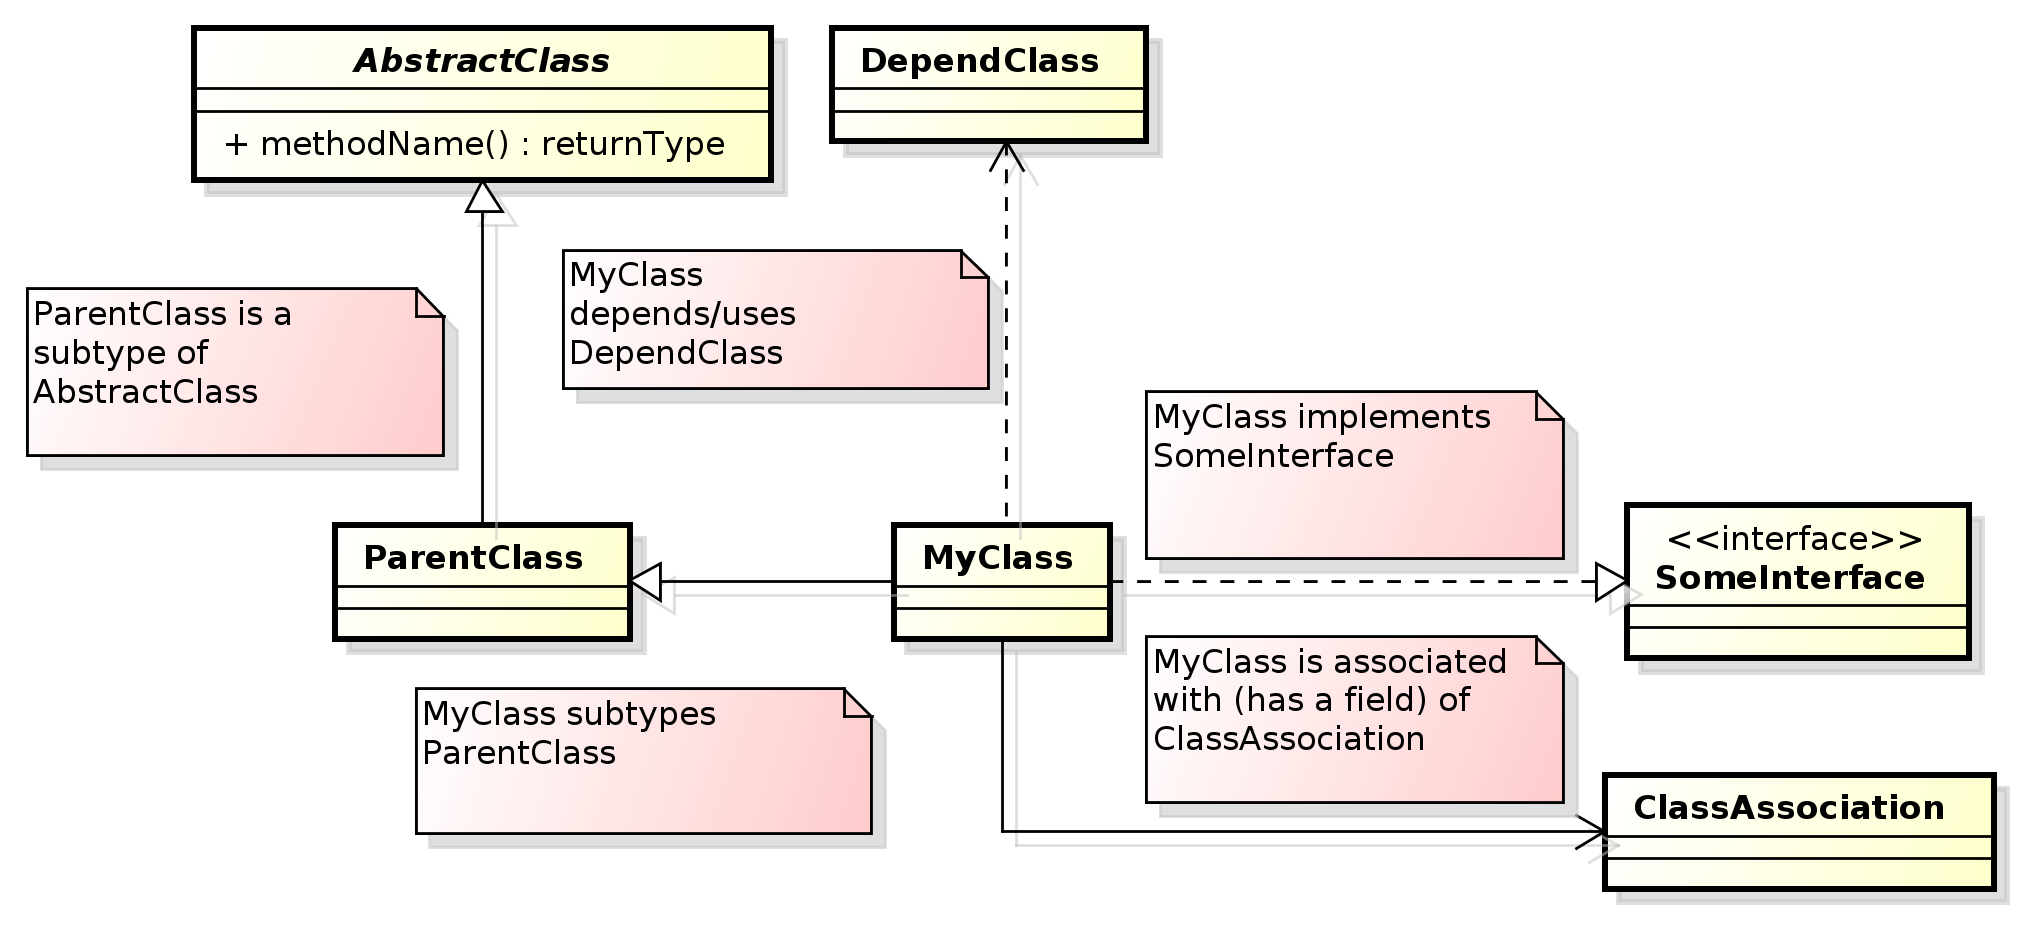
\includegraphics[scale=0.65]{img/UML/ClassDiagram.png}
\end{center}

The different arrow types mean different things as follows.

\begin{tabular}{c | l | l}
Relationship Type & Description & Example\\
\hline
\hline
Subtype & One class \texttt{extends} another & MyClass and Parent Class\\
Implements & One class \texttt{implements} an interface & MyClass and SomeInterface\\
Association & One class has a field for another class & MyClass and ClassAssociation\\
Dependency & One class uses another class & MyClass depends on DependClass.\\
\hline
\end{tabular}
~\\~
\\

\vspace{5pt}
One thing to keep in mind, is that these are logical distinctions and do not necessarily map to code. For example many dependency relationships are indeed stored as fields, but they aren't necessarily meant to be thought of as associations.




\subsection{Software Dependencies}

EALib is designed to introduce very little dependencies into codes that use aspect of it, (in other words it should be easy to use one part of EALib, without requiring others). One exception however is that almost all aspects of EALib are coupled to SLF4J \footnote{http://www.slf4j.org}, which is used for logging.

SLF4J is simply a front end and does not provide any logging functionality on it's own, EALib also includes logback \footnote{http://logback.qos.ch/} by default to do it's logging although this aspect can be replaced with log4j, java.util.logging, etc.

Different aspects of EALib depend on other libraries as follows:

\begin{tabular}{c c }
Name & Description  \\

\hline
\hline
Apache Commons Collections & Provides some new convenient collection types \\
Apache Commons I/O & Provides a Null Output Stream used for testing \\
Apache Commons Math & Provides Probability Distributions and other mathematical operations \\
Logback & 	Provides a default logging implementation for EALib \\
slf4J & Logging API that EALib links to \\
Spi & Provides an easy way to utilize the Service Provider Interface . \\
exp4j & Provides support for converting strings to formula, and evaluating them. \\
JCIP Annotations & Documents classes thread safety properties \\
OpenCSV & Used for parsing CSV Files \\
JCommander & Used for parsing Command line options\footnote{the version included is a custom and modified build of JCommander available here: https://github.com/SJrX/jcommander} \\
Guava & Used to provide an AtomicDouble class. \\ 
Numerics & Used to provide additional probability distributions and mathematical operations \\
Jama & Used to provide PCA Functionality used by the model. \\



\end{tabular}


\subsection{Design Principles and Conventions}

Certain conventions exist within EALib for a variety of reasons:

\begin{enumerate}

\item Most domain objects are entirely immutable. Those objects which aren't immutable, have generally been designed to have the bare minimum in mutability, for instance the \texttt{RunHistory} object has one method that modifies it's state, the \texttt{append()} method.

\item Most classes are related to each other through a design principle known as \emph{constructor based dependency injection}. In short, everything a class needs to operate is given to it, in its constructor. The aim is to allow the code to be much more flexible, by decoupling the object from it's dependencies. 

\end{enumerate}

\subsection{Order}

This document is primarily intended to be read in order, and there are few optional sections (even if the dependency isn't immediately apparent from the topics.

\subsection{Discrepancies and Errata}

This document's primary aim is to serve as an introduction to EALib and provide a high level overview of it's features and functionality. This document is not a complete description of the system, and in some cases only provides a brief description, and may be incorrect. The authoritative place to look is generally the code, and specifically the javadoc in the code. 

\subsection{Examples}

Within EALib there are several example applications that can be run out of the box and provide may provide some guidance on various features within EALib. The example applications are as follows

\subsubsection{Algorithm Test Utility}

This utility is used to test that a wrapper executes correctly, it is the best written example and almost every line is commented. It is the actual utility used in SMAC, and generally represents the best way of doing something, (in other words if it has a feature you want then you are best following the way it does it, even as opposed to another utility such as SMAC which may use older methods).

The location of the utility is at:\\ \texttt{ca.ubc.cs.beta.aclib.example.tae.TargetAlgorithmEvaluatorRunner}.

It has examples for the following:

\begin{enumerate}
\item Synchronous Target Algorithm Evaluation Execution.
\item Using Target Algorithm Evaluation Plugins.
\item Target Algorithm Evaluation Observation and Termination.
\item Parsing scenario files and getting domain objects.
\item Using JCommander to delegates and options.
\item Using JCommander to generate usage screens, and parse help options.
\item Logging
\end{enumerate}

\subsubsection{State Merge Utility}

This utility is used to merge various state files (files that store a series of runs, generally but not exclusively for an automatic configurator). Unfortunately some aspects of this, use less refined parts of EALib but it is still instructional.


The location of the utility is at:\\ \texttt{ca.ubc.cs.beta.aclib.example.statemerge.StateMergeExecutor}.

It has examples for the following:

\begin{enumerate}
\item Using and manipulating State Files.
\item Using the Random Forests built into EALib
\item Parsing scenario files and getting domain objects.
\item Using JCommander to delegates and options.
\item Using JCommander to generate usage screens, and parse help options.
\item Logging
\end{enumerate}


{\Large \textsc{Warning:}} The code for accessing models is actually really poor at this point. A rewrite is planned soon, but if you are unfortunate enough to have to deal with models presently than my advice to you is to simply copy and paste the \texttt{StateMergeModelBuilder} class, and hope it does what you want.

\subsubsection{Virtual Best Solver}

\textbf{TO DO}

\subsubsection{Random Target Algorithm Evaluator}

If you are looking for inspiration on how to implement your own Target Algorithm Evaluator, the place to start is probably looking at the classes in the package: \\
\texttt{ca.ubc.cs.beta.aclib.targetalgorithmevaluator.base.random}.

This target algorithm evaluator simply provides random responses to requests. Depending on what you are doing it may be all you need, unfortunately there are some limitations:

\begin{enumerate}
\item Because random results are generated instantaneously out of thin air, there is no delay and no support for observation. While if you look carefully you can see that it can simulate delays and observations, this handled by another set of decorators, and unfortunately these two decorators are perhaps the two most complicated decorators currently.
\item It isn't a realistic example of a TAE that should have high concurrent performance, it essentially creates a thread for every asynchronous execution which scales poorly.
\item It doesn't provide any guidance for thread safety which is important for TAEs.
\end{enumerate}

As a rule if you would like to or need to implement a TargetAlgorithmEvaluator then you either need to be very familiar with Thread Safety, but in some cases you can simply follow the Random example. If your TargetAlgorithmEvaluator needs to maintain any state, or invokes any \texttt{native} methods, it should make the \texttt{evaluateRuns()} method \texttt{synchronized}.

Final note is that you will also need to see {\Large \textbf{INSERT SECTION}} for information about how to create a project and load it into another EALib project.


\section{Wrapper Format}
\label{wrapper}
A \emph{wrapper} is a small script that sits between an EALib program and the target algorithm being evaluated. This allows users to easily supply scripts to execute their target algorithms without having to write a bunch of Java. 

EALib grew organically around the wrapper format used by Automatic Configurators such as ParamILS and SMAC, and it plays a key part to the abstractions in EALib, so it is good to be familiar with it. The conventions follow two parts governing invocation and output.

\subfile{wrapper}


\subsection{Glossary}



\section{Domain Objects}

\subsection{Introduction}

Domain objects represent various abstractions in EALib. They primarily are designed to be lightweight and are entirely focused on representing the information needed in the \ref{wrapper} section.

\subsection{Parameter Configuration Spaces}

Parameter Configuration Spaces are represented by two objects. \textbf{ParamConfigurationSpace} represents the entire set of allowable configurations. \textbf{ParamConfiguration} represents a point within that space:

\begin{center}
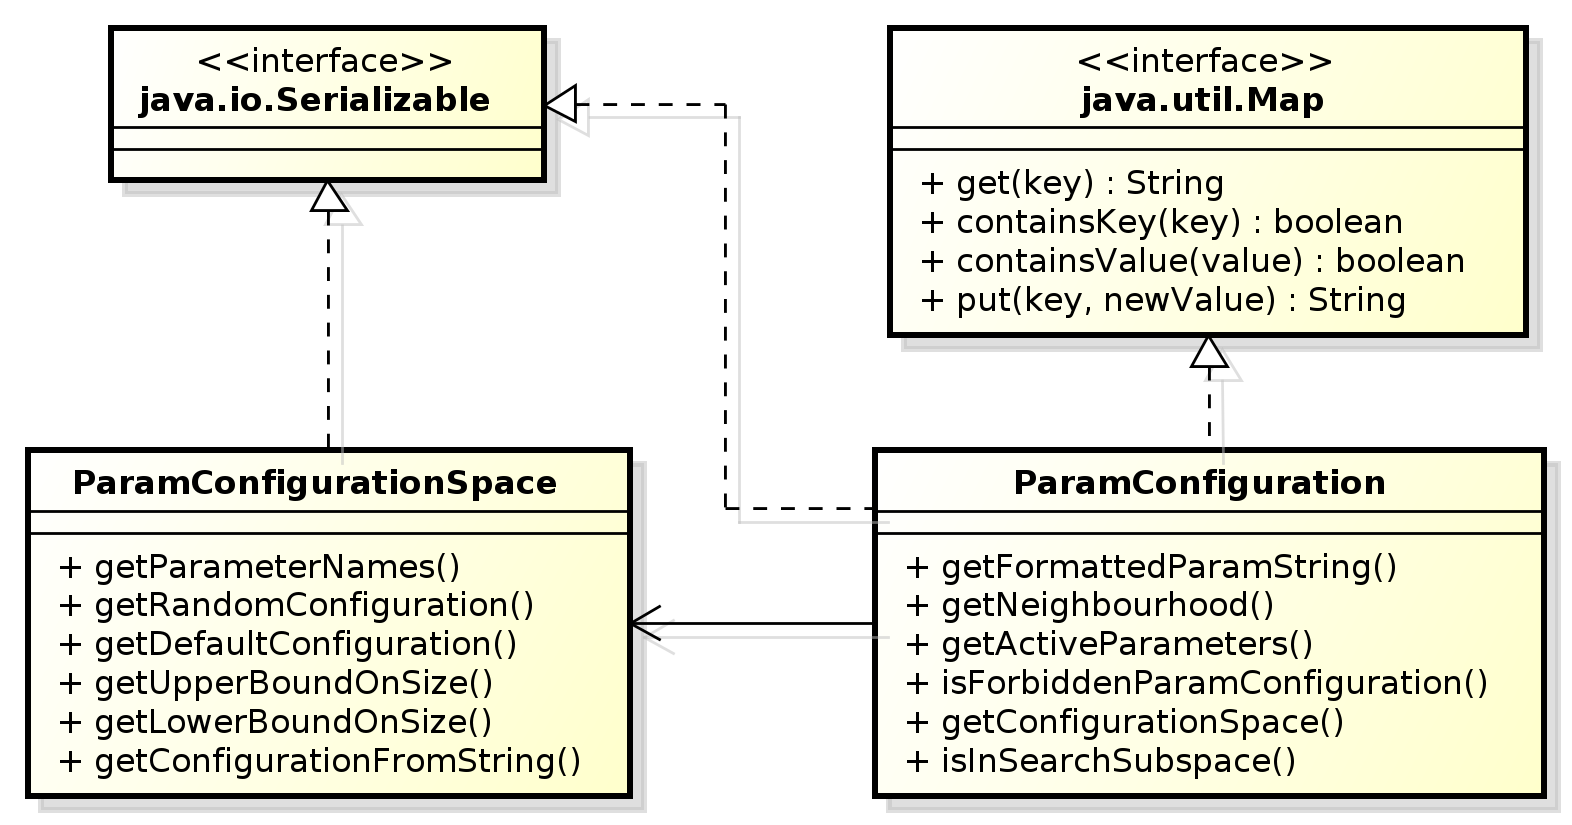
\includegraphics[scale=0.75]{img/UML/ConfigurationSpace.png}
\end{center}


The set of allowable parameter configuration spaces is complicated, one can read "The PCS File Format" for a full detailed specification of what is allowed to be represented. In short Parameter Configurations support name / value pairs like a standard Map with the following caveat:

\begin{itemize}
\item Parameter settings inherit from \texttt{Map} but they don't implement all the methods, additionally some of the semantics are different for example you cannot remove a key, the size of the map is always constant, and all the values have to come from the domain of the key. \footnote{In retrospect ParamConfiguration shouldn't inherit from Map}.
\item Some parameters can be conditional on the values of other parameters, the Map always contains active and inactive parameters however.
\item Parameter Settings can be Forbidden.
\item When getting Random Configurations from a Space, you will never get forbidden configurations generated.
\item \texttt{ParamConfiguration} objects have an ID, but this ID is used only for the local process and by convention is written in hex, and it simply represents that particular instance in memory, nothing prevents two objects with different IDs from being equal. Whenever a put() method is called on the Map, the ID is regenerated. 

\end{itemize}

\subsubsection{Construction}
\begin{description}
\item[ParamConfigurationSpace] are constructed directly , the primary input is the name of the file on disk that contains the specification according to the PCS File Format guide. Other constructors allow for hard coding the PCS file in memory. The \texttt{ParamFileHelper} method has some other methods that can construct instances.
\item[ParamConfiguration] are constructed from the \texttt{ParamConfiguration} class, namely the methods \texttt{getDefaultConfiguration()}, \texttt{getRandomConfiguration()}, \texttt{getConfigurationFromString()} among others. The only constructor visible is the copy constructor.
\end{description}

\subsubsection{Equality}
\begin{description}
\item[ParamConfigurationSpace] has equality defined as the absolute filename of the source file being equal. This isn't ideal, and when no file exists it is just a randomly generated string that gets used which is less than ideal at present.
\item[ParamConfiguration] has equality defined as the active parameters have equal values and both coming from equal \texttt{ParamConfigurationSpace} objects.
\end{description}

\subsubsection{Mutability and Thread Safety}

\begin{description}
\item[ParamConfigurationSpace] is immutable and consequently thread safe.
\item[ParamConfiguration] is mutable and is not technically thread safe. If objects are merely constructed from the \texttt{ParamConfigurationSpace} object however and then never modified again, then additional synchronization is generally not needed and the objects can be passed around without issue. 
\end{description}




\subsection{Problem Instance}


\begin{center}
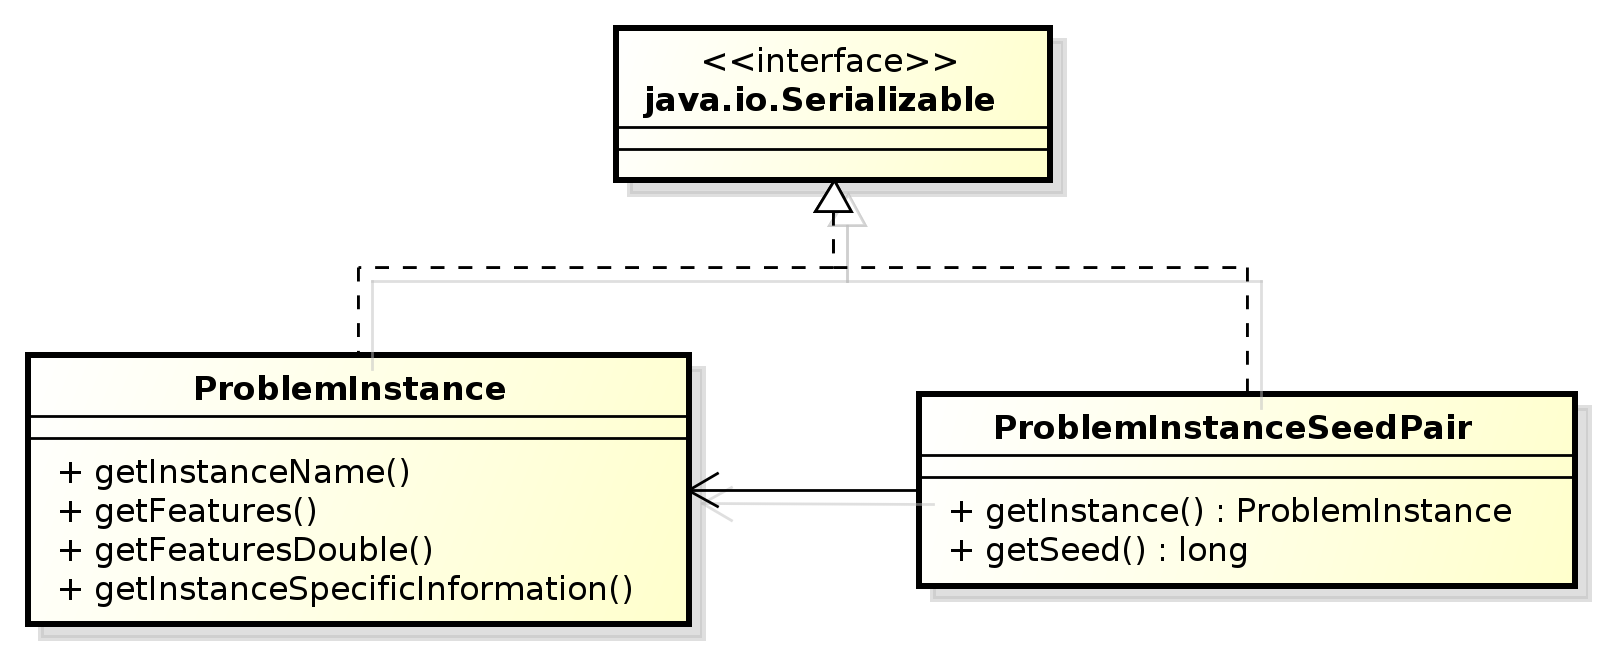
\includegraphics[scale=0.75]{img/UML/pi.png}
\end{center}

\texttt{ProblemInstance} objects represent the abstract problem instance that an algorithm will be run on. For example which particular SAT instance to use. They are very simple but there is a few caveats.

A \texttt{ProblemInstanceSeedPair} object is a container for a \texttt{ProblemInstance}




\begin{itemize}
\item The instance name is generally a file name but this is only a convention and nothing in EALib mandates that the instance exists.
\item Instances can have features, for using machine learning models, associated with them. At this point only continuous features are supported.
\item \textsc{WARNING} Instances currently also have the concept of an instance id. Relying on this is highly discouraged as it is generally brittle (it prevents you from merging different instance sets, or generating instances on the fly). Currently SMAC relies on this feature, but in general it only causes headaches, and will be removed eventually.

\end{itemize}

\subsubsection{Construction}
\begin{description}
\item[ProblemInstance] objects can be constructed directly with all needed information passed in a publicly available constructor.
\item[ProblemInstanceSeedPair] objects can be constructed directly with all needed information passed in a publicly available constructor.
\end{description}


\subsubsection{Equality}
\begin{description}
\item[ProblemInstance] has equality defined as the instanceName being equal.
\item[ProblemInstanceseedPair] has equality defined as both the \texttt{ProblemInstance} and the seed being equal.
\end{description}

\subsubsection{Mutability and Thread Safety}
\begin{description}
\item[ProblemInstance] is immutable and consequently thread safe.
\item[ProblemInstanceSeedPair] is immutable and consequently thread safe.
\end{description}


\subsection{Run Configurations}

\texttt{RunConfiguration} objects represent the logical view of what is being executed, that is ignoring the details of where the algorithm is on disk, what are the details that an EALib program cares about. It is a container object for the previous objects.

\begin{center}
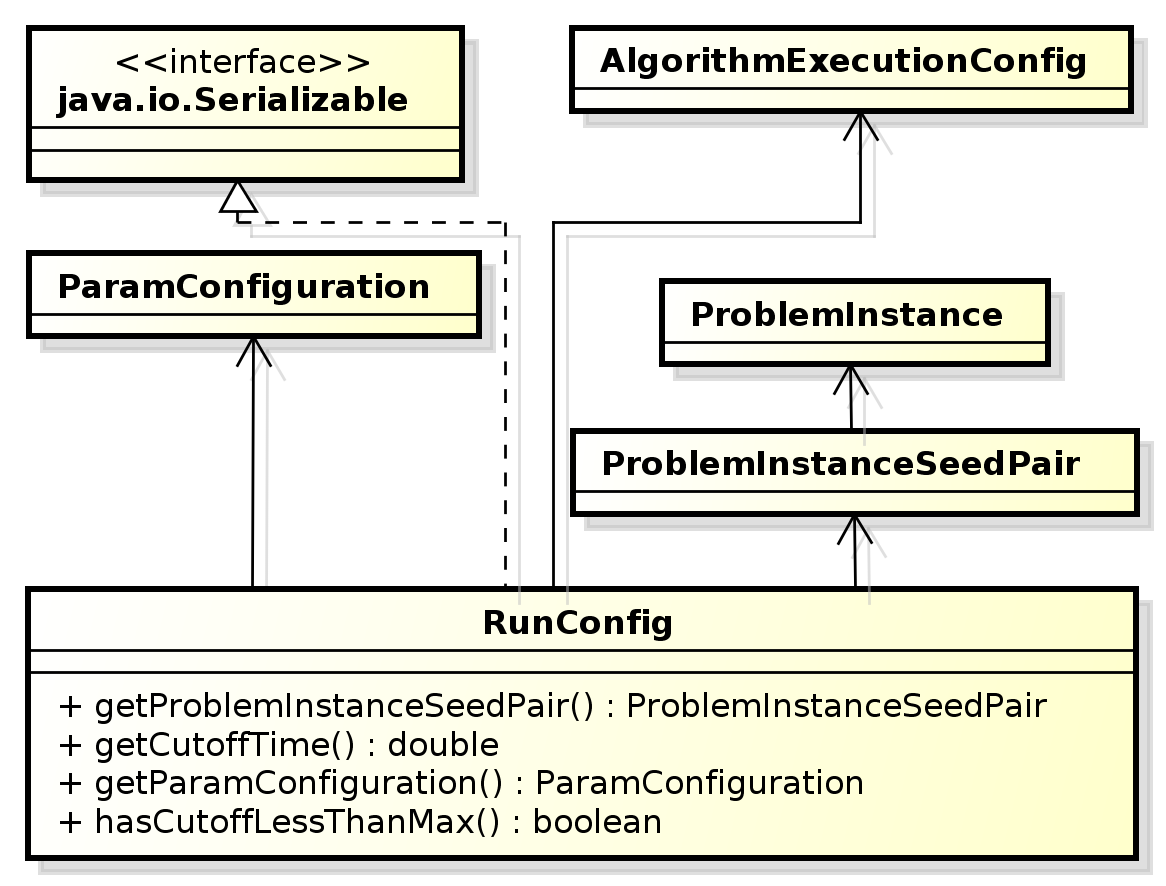
\includegraphics[scale=0.75]{img/UML/RunConfig_2.png}
\end{center}

\begin{itemize}
\item In future versions, the \texttt{RunConfiguration} object will also point to the \texttt{AlgorithmExecutionConfiguration} object.
\item One common source of confusion is what capping is. In EALib a run is considered 'capped' if it's cutoff time is less than cutoff time in the \texttt{AlgorithmExecutionConfig} and it reported \textbf{TIMEOUT} or \textbf{KILLED}. Another meaning is that it just needs to be \textbf{TIMEOUT} or \textbf{KILLED}.
\end{itemize}

\subsubsection{Construction}
\begin{description}
\item[RunConfiguration] objects can be constructed directly with all needed information passed in a publicly available constructor.
\end{description}


\subsubsection{Equality}
\begin{description}
\item[RunConfig] has equality defined as all the fields being equal.
\end{description}

\subsubsection{Mutability and Thread Safety}
\begin{description}
\item[RunConfig] immutable and consequently thread safe, subject to the proviso of the \texttt{ParamConfiguration} object.
\end{description}

\subsection{Algorithm Execution Configuration}

\texttt{AlgorithmExecutionConfiguration} objects represent the ``physical'' information about executing an algorithm, namely where the algorithm is, and what type it is.

\begin{center}
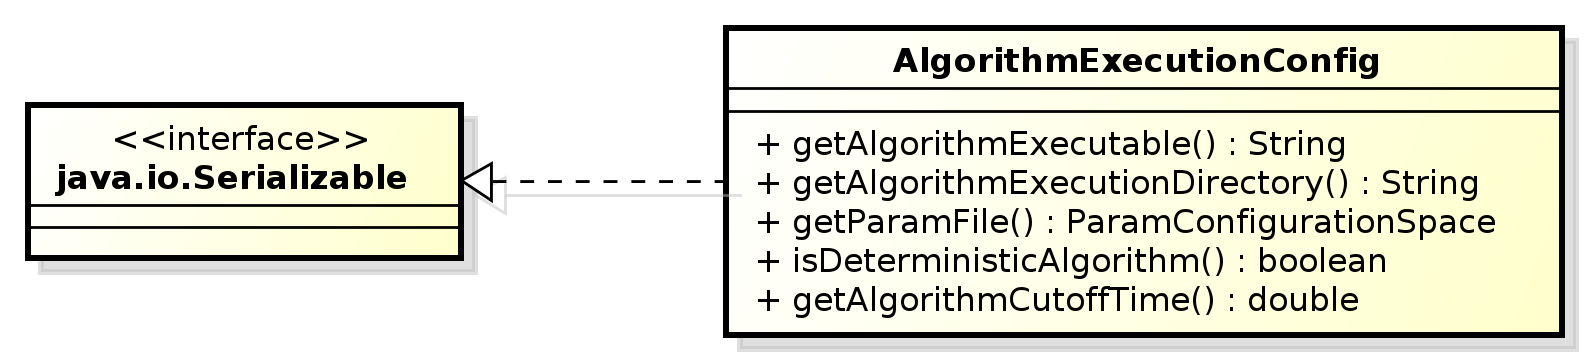
\includegraphics[scale=0.75]{img/UML/ExecConfig.png}
\end{center}

\begin{itemize}
\item Currently the object also has an \texttt{executeOnCluster} property which doesn't serve any useful purpose at all.
\item the \texttt{getParamFile()} method reflects a previous name of the \texttt{ParamConfigurationSpace} class.
\end{itemize}

\subsubsection{Construction}
\begin{description}
\item[AlgorithmExecutionConfiguration] objects can be constructed directly with all needed information passed in a publicly available constructor.
\end{description}


\subsubsection{Equality}
\begin{description}
\item[AlgorithmExecutionConfig] has equality defined as all the fields being equal.
\end{description}

\subsubsection{Mutability and Thread Safety}
\begin{description}
\item[AlgorithmExecutionConfig] immutable and consequently thread safe, subject to the proviso of the \texttt{ParamConfiguration} object.
\end{description}

\subsection{Algorithm Run} 

\texttt{AlgorithmRun} objects represent the output of a wrapper execution, and provide accessor methods to obtain those methods. It subtypes \texttt{java.util.Runnable}, but this is primarily an internal detail used during construction.

\begin{center}
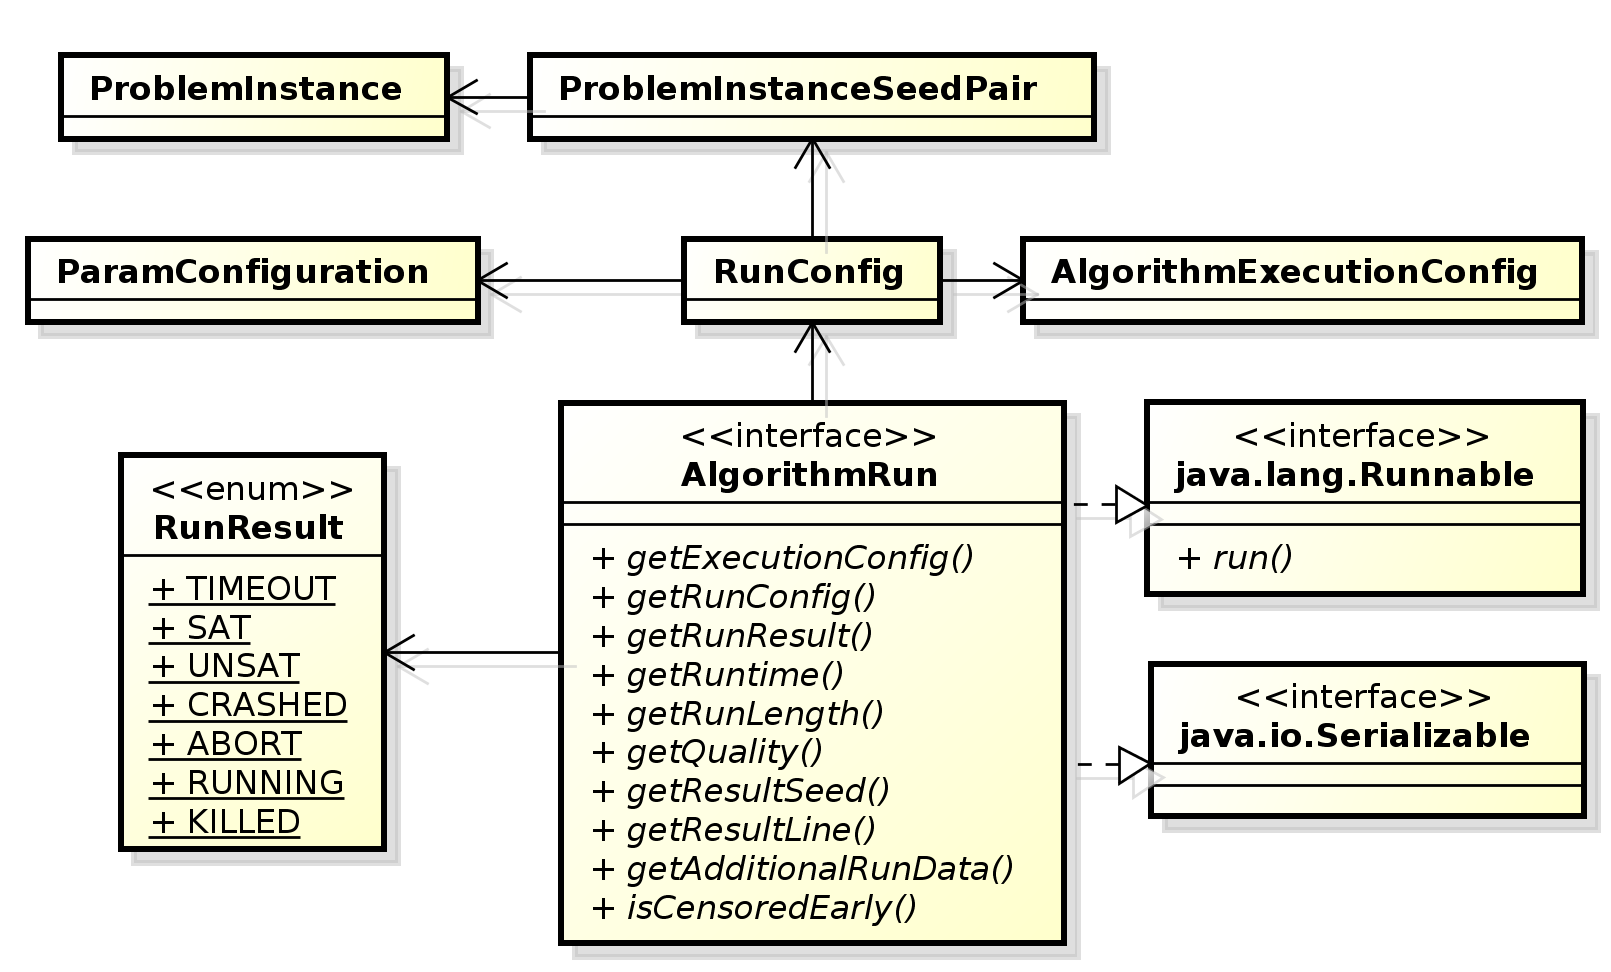
\includegraphics[scale=0.75]{img/UML/AlgorithmRun.png}
\end{center}

\begin{itemize}
\item It is generally expected that outside of the \texttt{TargetAlgorithmEvaluator} objects that the \texttt{AlgorithmRun} object only represents a snapshot of a completed / running run. The \texttt{run()} method should be a noop for almost all users.
\item  Not shown, but the \texttt{AlgorithmRun} interface also implements the \texttt{java.util.Callable<Object>} interface. Invoking \texttt{call()} must be the same as invoking \texttt{run()}. 
\end{itemize}

\subsubsection{Construction}
\begin{description}
\item[AlgorithmRun] objects are interfaces and there is no standard way of constructing them. In general these objects are retrieved from a \texttt{TargetAlgorithmEvaluator} \ref{sec:tae}. One subtype \texttt{ExistingAlgorithmRun} has a publicly accessible constructor.
\end{description}
\subsubsection{Equality}
\begin{description}
\item[AlgorithmRun] has equality defined as the \texttt{AlgorithmExecutionConfiguration} and the \texttt{RunConfiguration} object being equal. In particular note that it does not depend at all on the output. 
\end{description}

\subsubsection{Mutability and Thread Safety}
\begin{description}
\item[AlgorithmExecutionConfig] immutable and consequently thread safe, subject to the proviso of the \texttt{ParamConfiguration} object.
\end{description}


\section{Options \& JCommander}

EALib utilizes JCommander which makes handling command line arguments incredibly easy. While technically your application doesn't need to use JCommander, it is generally recommended as it is very powerful. You should read http://jcommander.org/ for an introduction to JCommander.





\subsection{Modifications to JCommander}

{\Large \textsc{Warning} }:The version of JCommander used in EALib is modified, and probably slightly out of date the official version, the source for our build of JCommander is available from https://github.com/SJrX/jcommander.

Differences:
\begin{enumerate}
\item Our version supports a new annotation type \texttt{@ParameterFile}, on \texttt{@Parameter} parameters, this signifies that the parameter value should be read as a file (in Java Properties File Format \footnote{See: http://docs.oracle.com/javase/tutorial/essential/environment/properties.html}). The property file is first escaped so that \textbackslash isn't interpreted as an escape character. 

\item Boolean variables generally have arity 1, which means you must specify true and false for those parameters.
\end{enumerate}

\subsection{Example}

Options objects are very simple, they consist of a bunch of fields with special annotation, you are encouraged to look in the examples in Section \ref{sec:examples}, but here is a very primitive example of what an Option object looks like (with some custom extensions).


\definecolor{mygreen}{rgb}{0,0.6,0}
\lstset{language=Java, showspaces=false,showstringspaces=false, keywordstyle=\color{purple},identifierstyle=\color{blue},
  stringstyle=\color{mygreen}}
  
\definecolor{javared}{rgb}{0.6,0,0} % for strings
\definecolor{javagreen}{rgb}{0.25,0.5,0.35} % comments
\definecolor{javapurple}{rgb}{0.5,0,0.35} % keywords
\definecolor{javadocblue}{rgb}{0.25,0.35,0.75} % javadoc
 
 
\lstset{language=Java,
basicstyle=\ttfamily,
keywordstyle=\color{javapurple}\bfseries,
stringstyle=\color{mygreen},
commentstyle=\color{mygreen},
morecomment=[s][\color{javadocblue}]{/**}{*/},
numberstyle=\tiny\color{black},,
numbersep=10pt,
tabsize=4,
showspaces=false,
showstringspaces=false}

  
  
\begin{small}
\begin{lstlisting}[]
@UsageTextField(title="MyOptions", description="Example options object", noarg=Foo.class)
class MyOptions extends AbstractOptions{

	@UsageTextField(defaultValues="1 if deterministic 10 otherwise"}
	@Parameter(names="--challenges", description="This is an example command")
	public int challenges;
	
	@ParametersDelegate 
	public HelpOptions help = new HelpOptions();

	@UsageTextField(level=OptionLevel.ADVANCED}
	@Parameter(names="--debug", description="Show debug information")
	public boolean debug;

	@ParameterFile
	@Parameter(name="--challenges-file", description="file to read information from")
	public File defaultFile
}
\end{lstlisting}
\end{small}

The \texttt{@UsageTextField} option is another annotation that is used for additional information when ever we need to display these options for users, for example in a usage screen or in a \LaTeX manual. 

\begin{enumerate} 
\item When tagged on a class, you can set the title and description that will be displayed, you can also set a class (in the above Foo.class), that will be called if the application is supplied without any arguments. This class has to be a subtype of:\\ \texttt{ca.ubc.cs.beta.aclib.misc.options.NoArgumentHandler}

\item You can use it to set the level at which the option will be displayed, for instance --debug will only be displayed if the user is requesting ADVANCED or DEVELOPER options.

\item You can override thing like the default value that will be displayed (normally computed by looking at the current value). You can also override the domain that will be set.
\end{enumerate}


\subsection{Type restrictions}

All Option objects as subtypes in EALib, are restricted to be subtypes of the type \texttt{AbstractOptions}.
\begin{center}
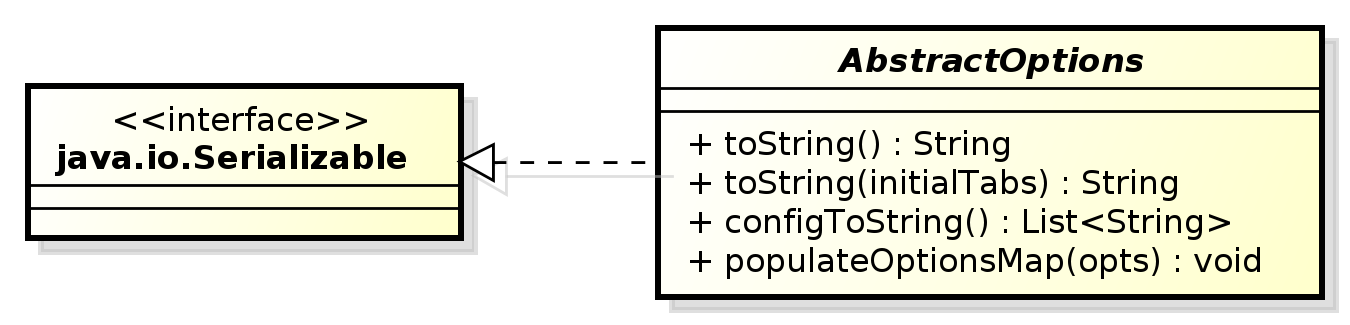
\includegraphics[scale=0.75]{img/UML/AbstractOptions.png}
\end{center}

There are two important operations provided by \texttt{AbstractOptions} the first is the \texttt{toString()} method provides a very friendly toString() method that handles delegates in a nice way. It also (if the field has the string ``password'' in it, the field will not be printed).

The second is \texttt{populateOptionsMap()} which takes all the values that are \texttt{@Parameter} and throws them in a map from the names() [sans first two dashes], to their value.

\subsubsection*{Serialization Warning}

The built in AbstractOptions objects do implement \texttt{java.io.Serializable} but there are no guarantees about the representations being particularly stable between versions. The Serializability is primarily to aid distributing options in a distributed setting running under the exact same version. 

\subsection{Parsing Existing File Formats}

There are many existing file formats used by various projects written in EALib some of them are the following.

\begin{description}
\item[PCS Files] which control the specification of the parameter space represented by the \texttt{ParamConfigurationSpace} object.
\item[Instance Files] which control the specification of instances, and what seeds to use on those instances.
\item[Feature Files] which list the features with associated instances.
\item[Scenario Files] which specify details about Automatic Configuration runs, and are used generally to specify Algorithms. Scenario Files generally contain all of the above.
\end{description}

Parsing these formats generally occurs through the use of a \texttt{@ParametersDelegate}. For example SMAC and the Validate utility have the following (simplified) delegate structure:

\begin{center}
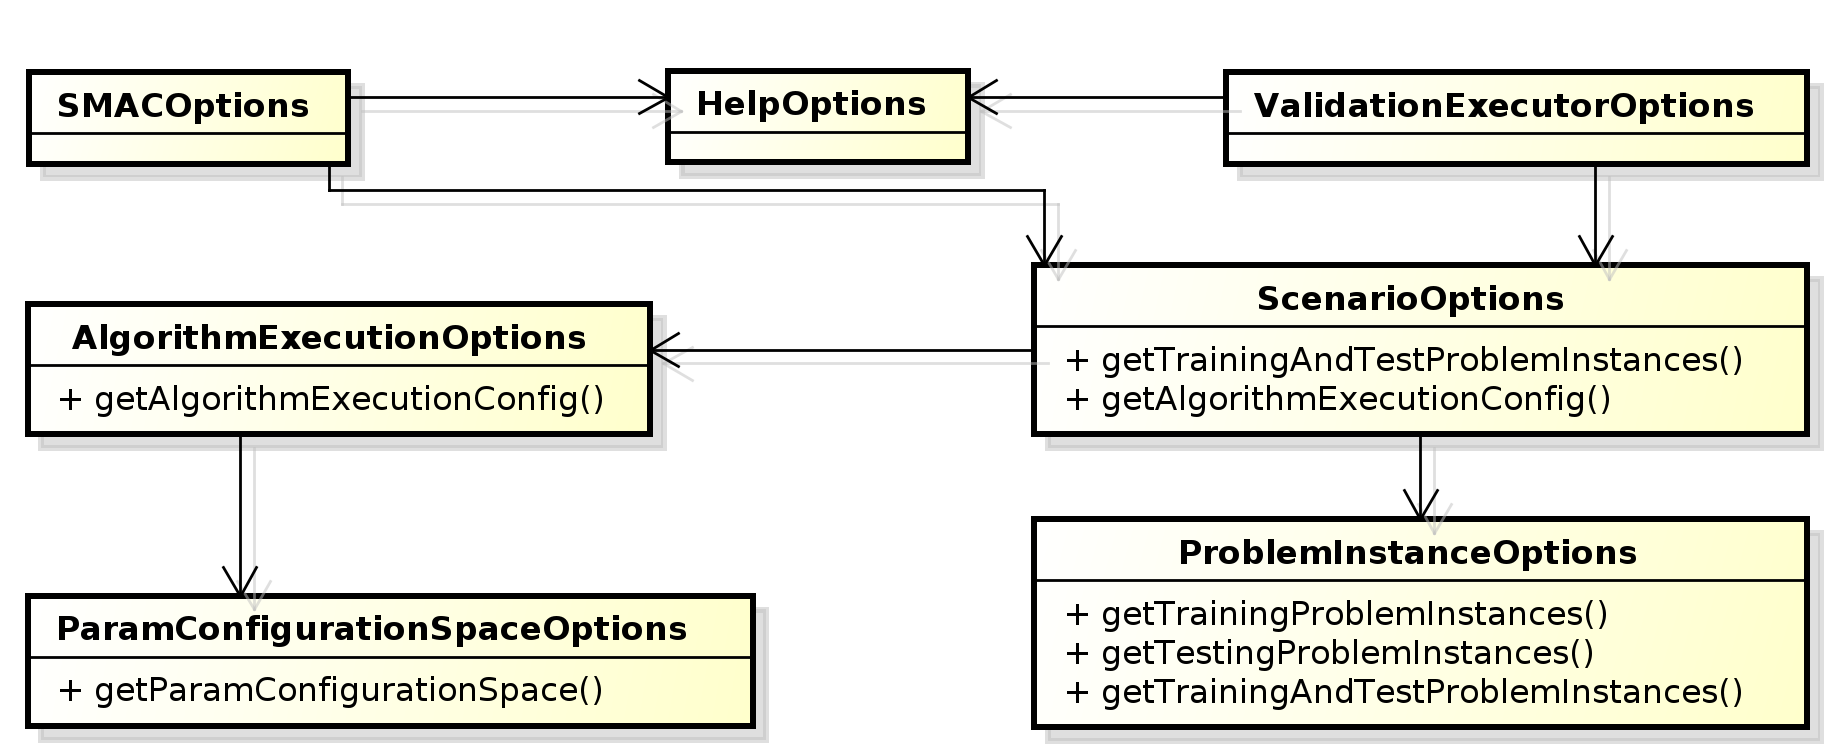
\includegraphics[scale=0.75]{img/UML/Options2.png}
\end{center}


To actually get the domain representation of objects, it's generally as simple as include the appropriate delegate, which will expose the necessary command line option, and then invoking the correct method on the delegate in question. Scenario options don't have a domain object, but have a file format outlined in the SMAC manual. This is handled through a \texttt{@ParameterFile} option.

\subsection{Coupling to JCommander}

It is important to note that you aren't actually coupled to using JCommander or making a command line utility. While you occasionally have to use pre-existing delegates to construct certain things (in most cases) you don't actually have to make a command line utility or invoke any code (although the JAR is required in your project).


\section{Target Algorithm Evaluator}
\label{sec:tae}
Target Algorithm Evaluation is probably the main reason you are using EALib to begin with. At a basic level it is the interface your code will use to invoke a wrapper, or as far as Domain Objects \ref{sec:domain} are concerned allow you to convert a \texttt{RunConfiguration} object to a \texttt{AlgorithmRun} object.
\begin{center}
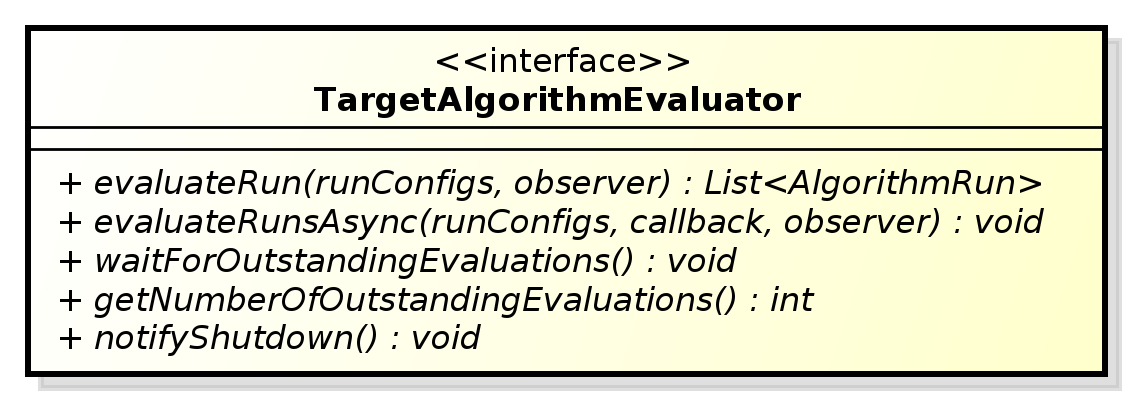
\includegraphics[scale=0.75]{img/UML/TAEBasic.png}
\end{center}
They are designed to be simple to use, very flexible and to work in highly concurrent applications.

You may find it handy to refer to refer to the examples outlined in \ref{sec:examples} as well as the Javadoc for the TargetAlgorithmEvaluator interface.

\subsection{Execution Methods}

Target Algorithm Evaluators support many different execution methods, that are useful in different contexts.

\subsubsection{Standard Execution}

Standard Execution is simply invoking the \texttt{evaluateRun(List<RunConfiguration>)} method, and when it returns it gives you a list of the associated \texttt{AlgorithmRun} objects.

Here is a sequence diagram just for warm up:

\begin{center}
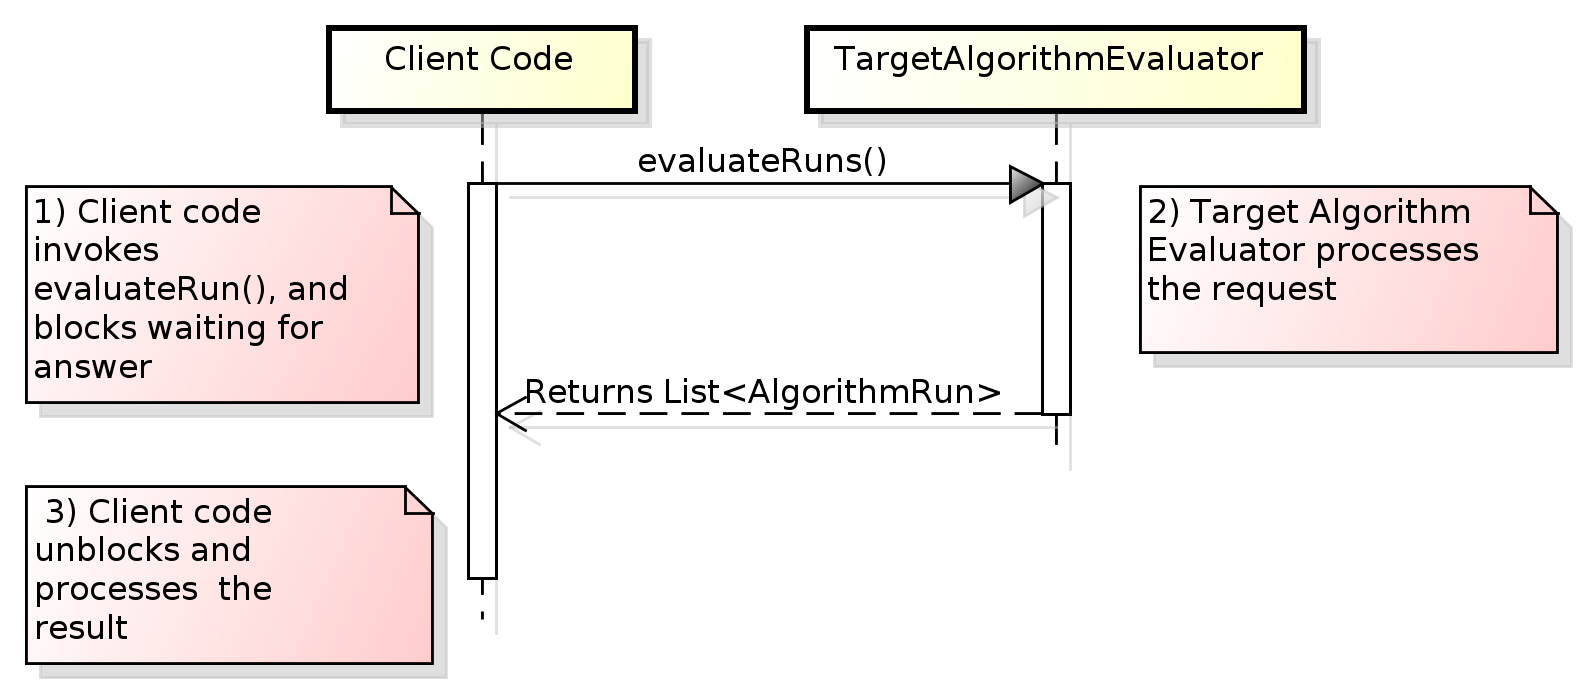
\includegraphics[scale=0.75]{img/UML/TAESequence1.png}
\end{center}

\subsubsection{Asynchronous Execution}

Standard Execution requires a thread for every concurrent request which can be VERY expensive. A different method that is invoked is the \texttt{evaluateRunAsync(List<RunConfiguration>, TargetAlgorithmEvaluatorCallback)} method where an instance of \texttt{TargetAlgorithmEvaluatorCallback} is provided with the list of runs to complete.

\begin{center}
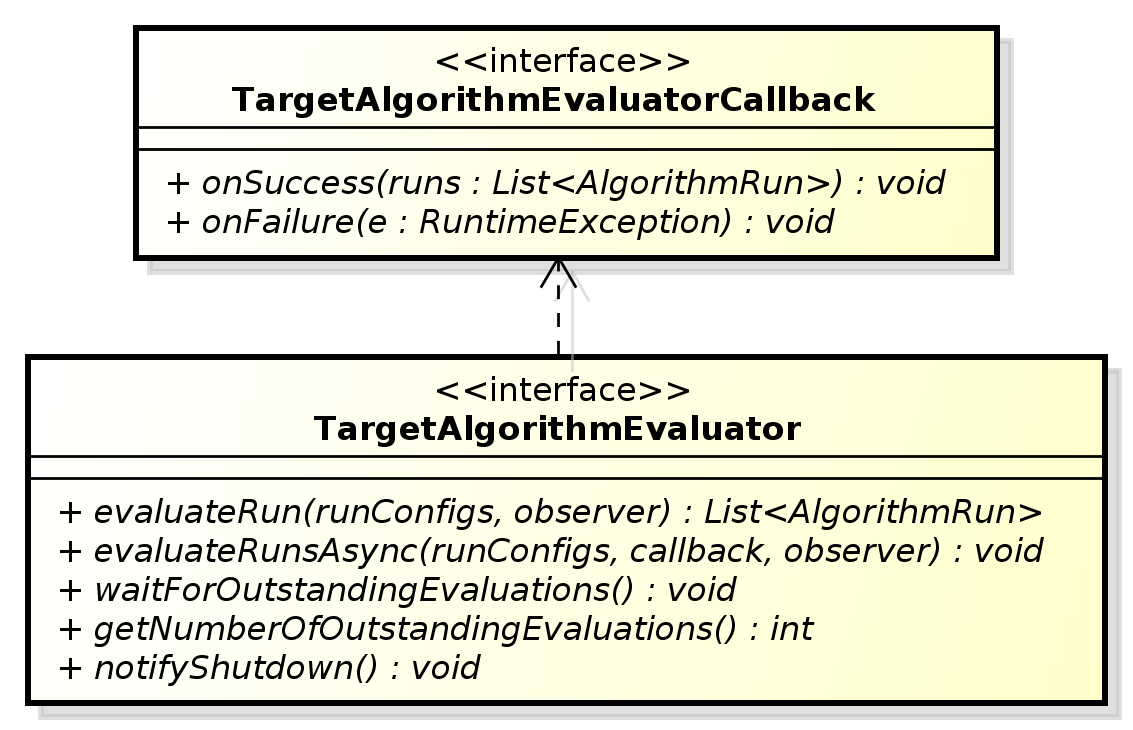
\includegraphics[scale=0.75]{img/UML/TAECallback.png}
\end{center}


If the runs complete successfully the \texttt{onSuccess()} method is called, if a RuntimeException occurs then \texttt{onFailure()} is called.


\begin{center}
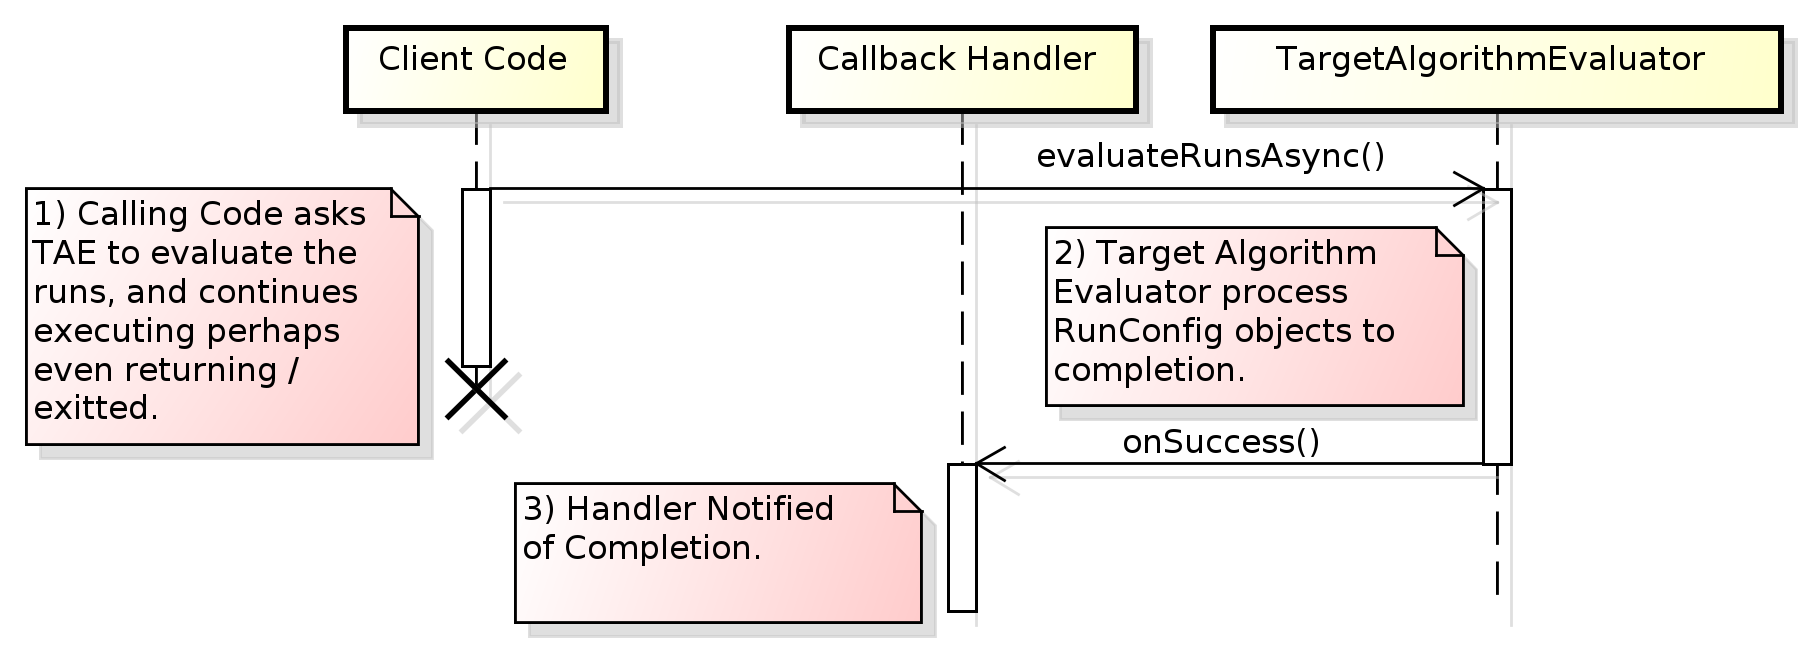
\includegraphics[scale=0.75]{img/UML/TAESequence2.png}
\end{center}


Generally this is the method with the best performance in concurrent applications, and the most scalable but the callback is invoked in another thread which requires an the callbacks to be written with thread safety in mind. 

Another limitation is that once the runs are dispatched you have no control over them, consider for example if you want to concurrently run a bunch of solvers and terminate when the first run is done, there is no way to do this in the above setup.

\subsubsection{Observation}

Target Algorithm Evaluators have a mechanism that allows you to observe the current status of a run, and optionally terminate it. Through the use of the \texttt{evaluateRuns(List<RunConfiguration>, TargetAlgorithmEvaluatorRunObserver)} and \texttt{evaluateRunsAsync(List<RunConfiguration>, TargetAlgorithmEvaluatorRunObserver)} methods.


\begin{center}
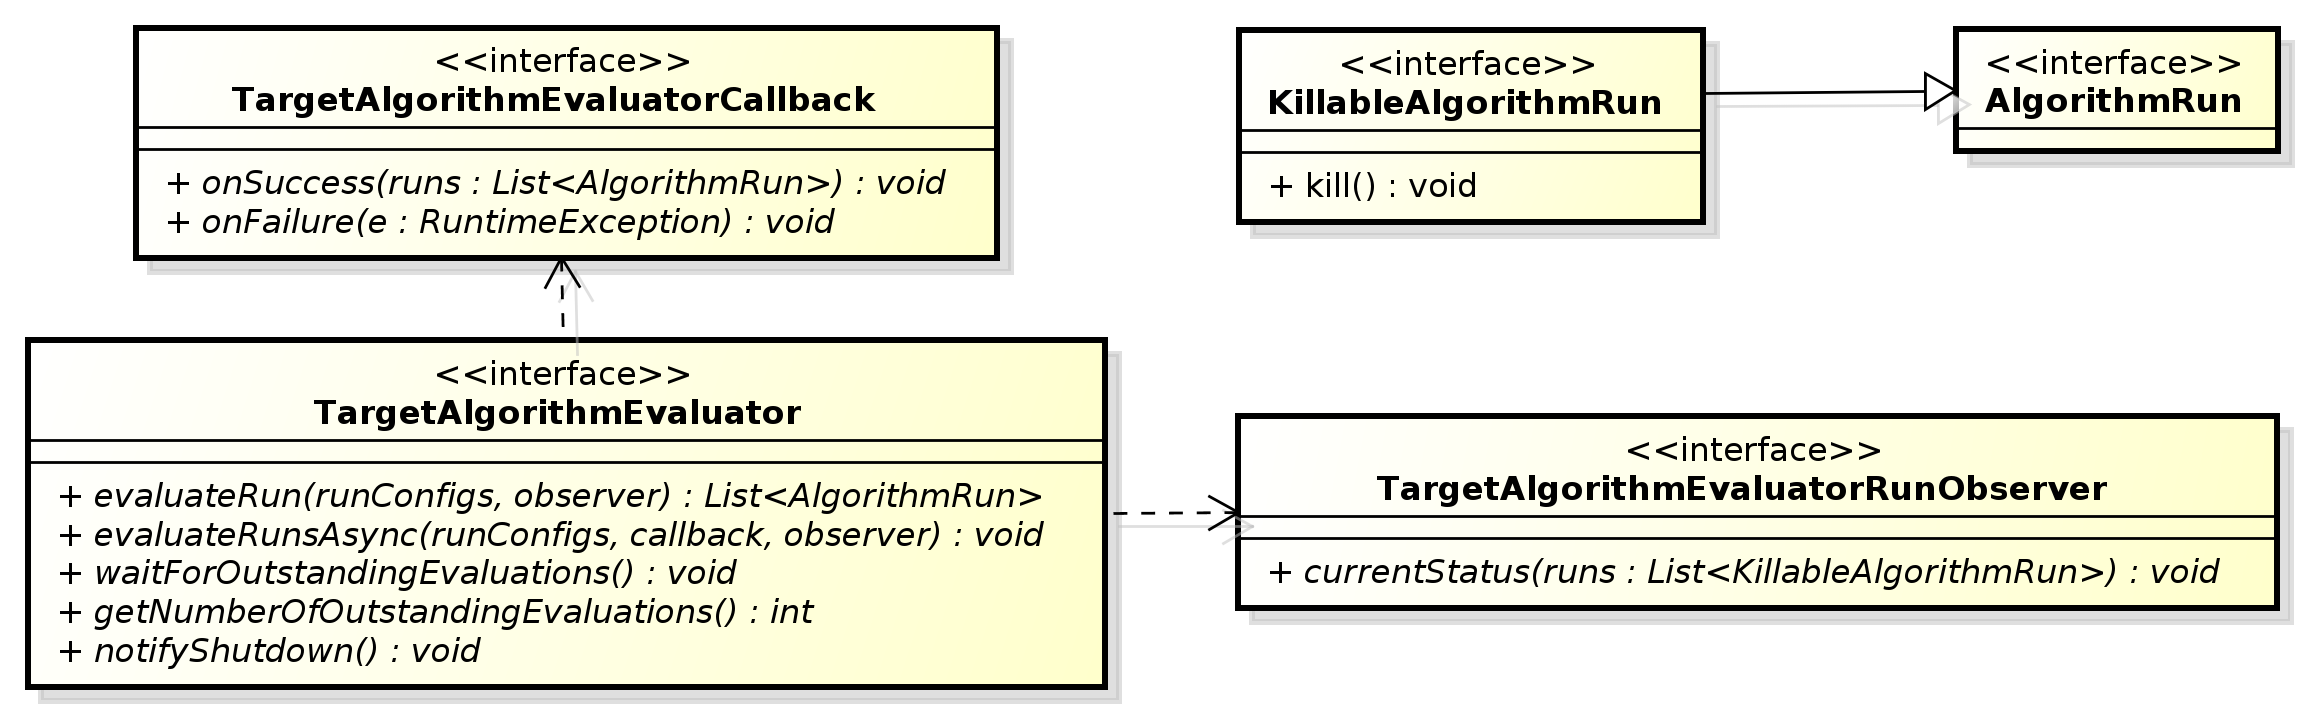
\includegraphics[scale=0.5]{img/UML/TAEObserver.png}
\end{center}


Note that the \texttt{currentStatus()} method takes \texttt{KillableAlgorithmRun} objects which are a subtype of the \texttt{AlgorithmRun} object.

When using observers you should bear in mind the following:
\begin{itemize}
\item The \texttt{getRunResult()} will return \texttt{RUNNING} if the algorithm is currently running. This is a snapshot however, and this object will not be updated, instead the \texttt{currentStatus()} method will be invoked again with new objects.

\item The observers are invoked on a best effort basis, not all \texttt{TargetAlgorithmEvaluator} will notify an observer, and those that do may not support termination.

\item The \texttt{kill()} method is done on a best effort basis, their is no guarantee that when or if the run will actually be terminated.

\item Runs in the batch that are completed will have there full results available, runs that are in \texttt{RUNNING} will only at best have their current \texttt{getRuntime()} and \texttt{getWallclockExecutionTime()} as accurate (and perhaps slightly delayed).

\item Observers may only provide approximate information about \texttt{RUNNING} runs, and it's possible that the \texttt{getRuntime()} and \texttt{getWallclockExecutionTime()} may decrease. Two examples where this can occur is if the run crashed and it is being re-run automatically, and the other is when \texttt{getRuntime()} is being approxmiated by the wallclock time. The wrapper may return a lesser value. If a run isn't in \texttt{RUNNING} then it should be authorative.

\item The observation happens in a separate thread, provided that you submit a unique observer for every batch, and the observer doesn't touch any shared state (only local state or is stateless), then this should be thread safe. If the observer has local state, and you want to share it between multiple concurrent runs you should make the \texttt{currentStatus()} method \texttt{synchronized}. In general you should not modify global state with an observer.

\end{itemize}

\pagebreak
Example Observer Code to terminate runs when the sum of the runtime is $>=$ 40 seconds:



\begin{center}
\begin{lstlisting}[]
class Observer extends TargetAlgorithmEvaluatorRunObserver {
	public void currentRunStatus(List<? extends KillableAlgorithmRun> runs) {
		double sum = 0;
		for(AlgorithmRun run : runs)
			sum+= run.getRuntime();
		
		if(sum > 40.0)	{
			for(KillableAlgorithmRun run : runs)
			{
				run.kill()
			}
		}
	}
}

\end{lstlisting}
\end{center}




\begin{center}
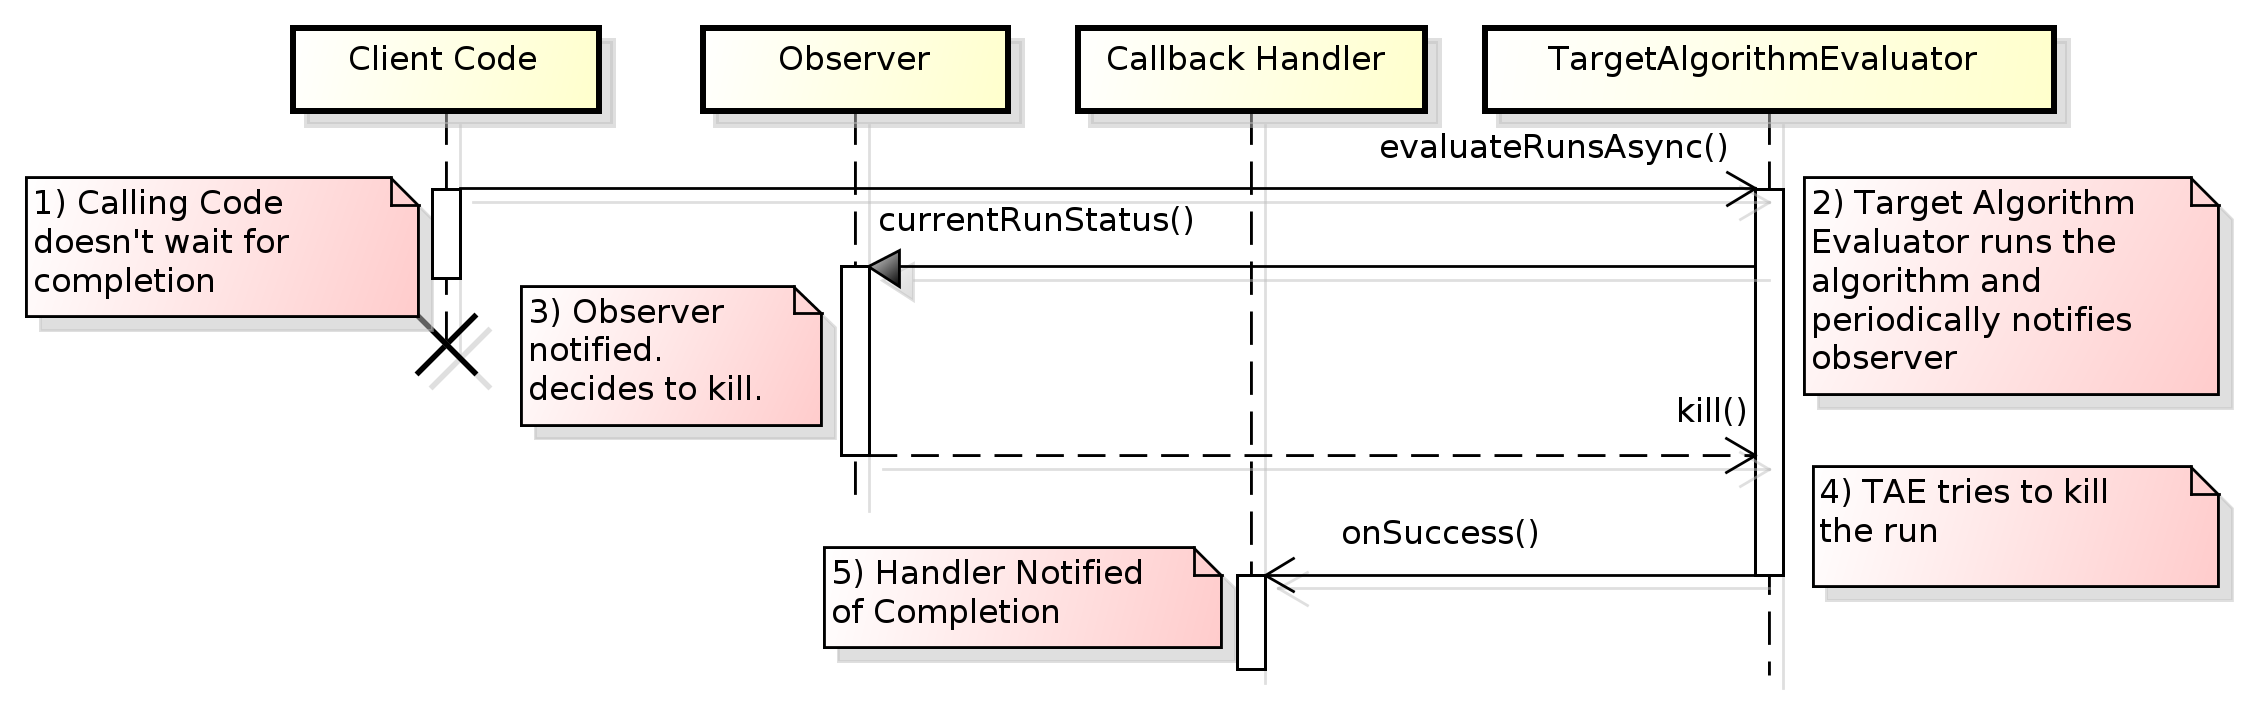
\includegraphics[scale=0.5]{img/UML/TAESequence3.png}
\end{center}


\subsubsection{TAE Queues}

While \ref{sec:async-exec} is the best performing mechanism, it does introduce much complexity 
on to you the developer. EALib supports one final execution mechanism that can provide asynchronous execution without the thread safety worries.

\begin{center}
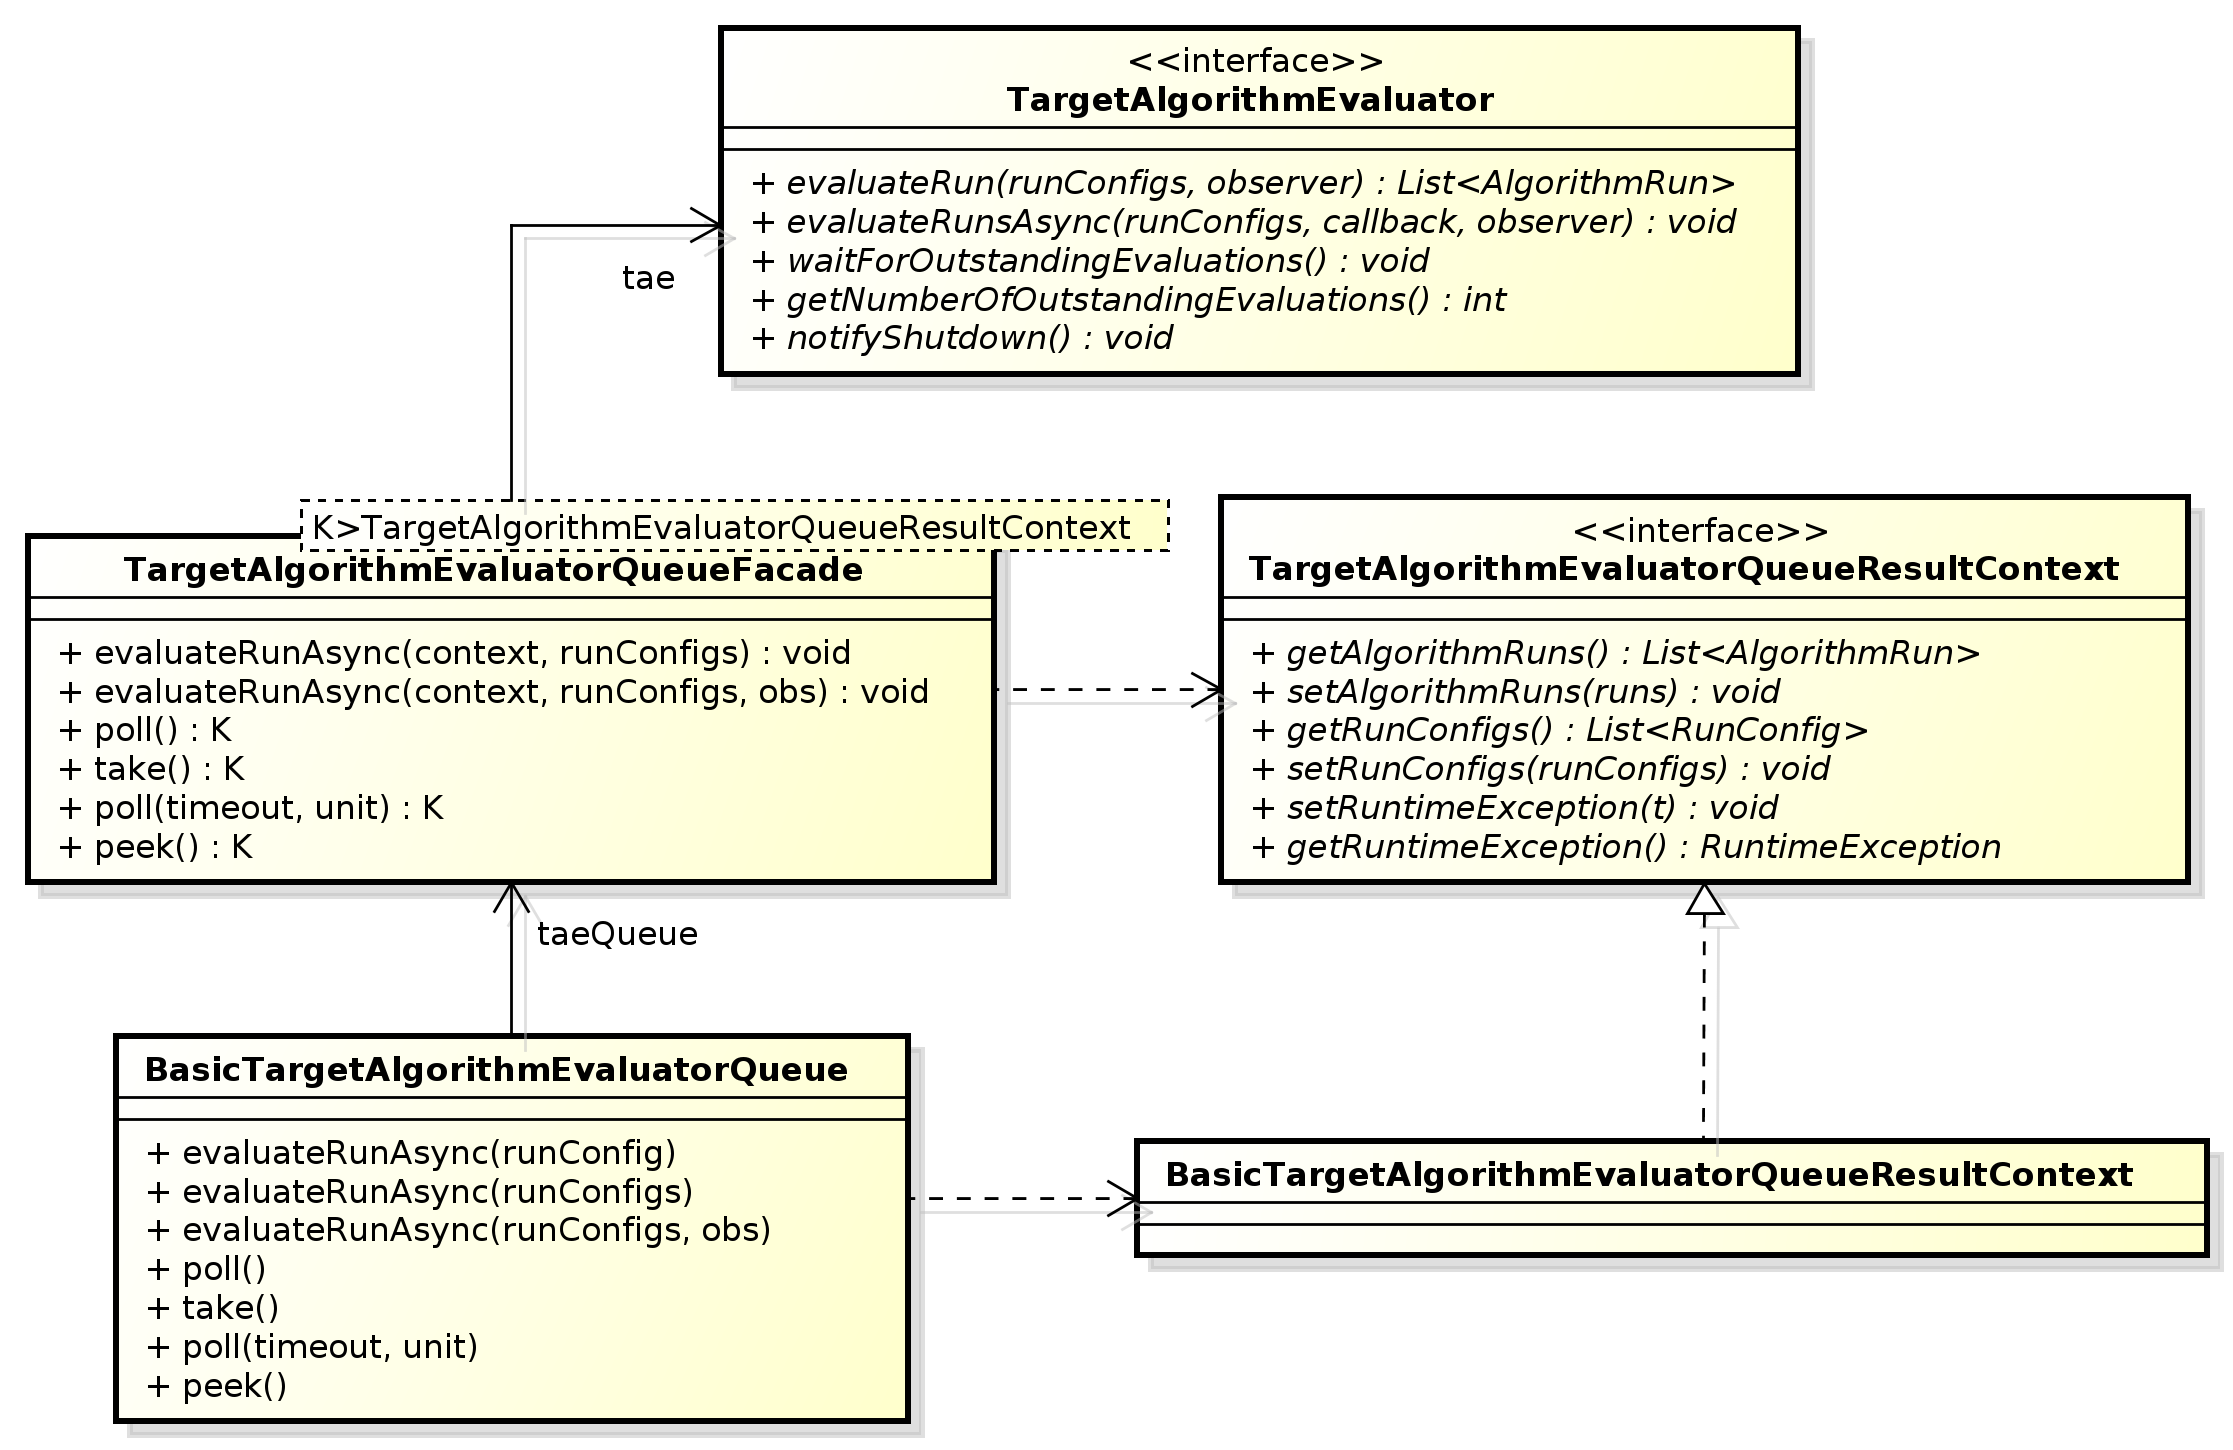
\includegraphics[scale=0.60]{img/UML/TAEQueue.png}
\end{center}

A simplified view of how the above works is as follows (the class diagram is more general which I will explain in a second), in the \texttt{BasicTargetAlgorithmEvaluatorQueue} the \texttt{evaluateRunsAsync()} methods are exposed, when cause the algorithm to start executing with a special callback that causes the results stored in the in a queue. These objects have type\\ \texttt{TargetAlgorithmEvaluatorQueueResultContext}, and as you can see roughly correspond to the information in a callback. The client code can then retrieve these objects from the queue via the \texttt{poll()}, \texttt{take()}, \texttt{peek()}, etc... methods.

The \texttt{BasicTargetAlgorithmEvaluatorQueue} doesn't allow client code to supply it's own client context, but it wraps a more general \texttt{TargetAlgorithmEvaluatorQueueFacade} which allows users to supply there own subtypes of \texttt{TargetAlgorithmEvaluatorQueueResultContext}. This allows you to easily keep tag runs with additional information you need when you want to process the results.

\begin{center}
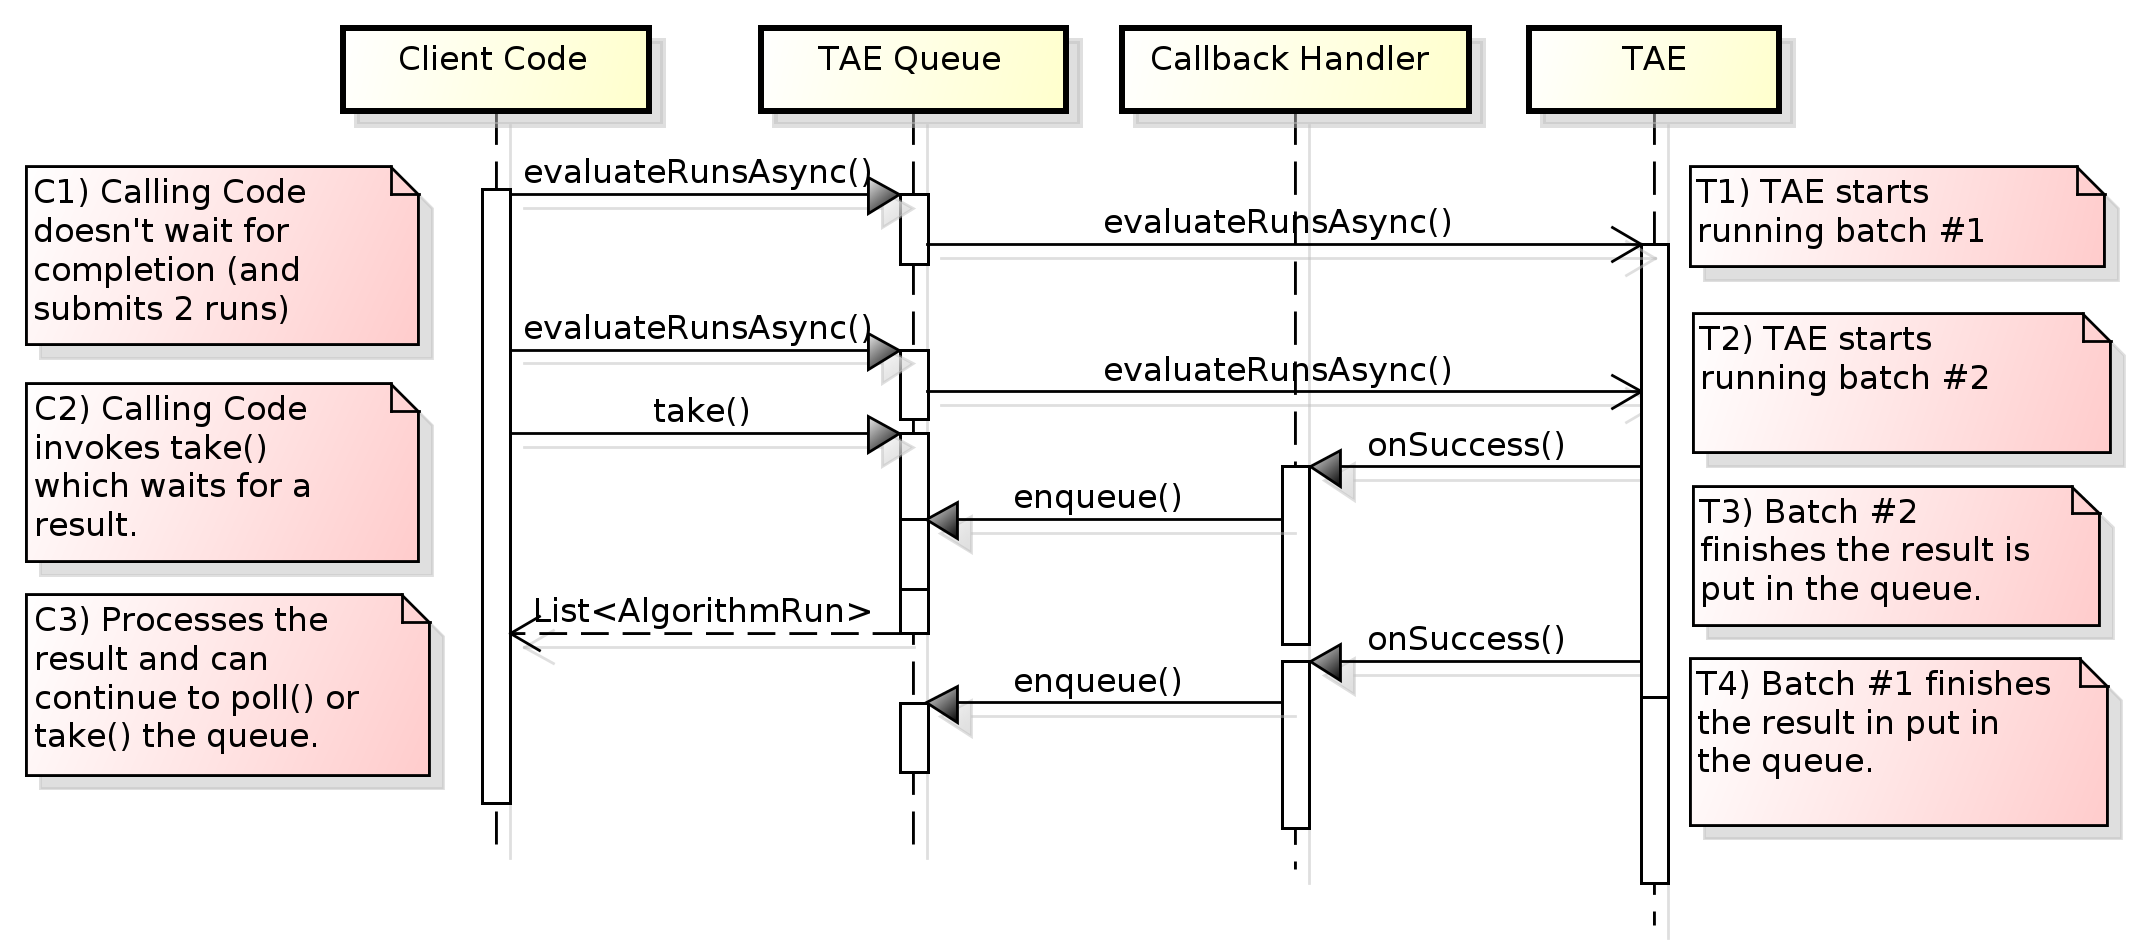
\includegraphics[scale=0.60]{img/UML/TAESequence4.png}
\end{center}

\subsection{Target Algorithm Evaluator Decoration}

One might wonder how failures and other common tasks are handled in EALib, is it up the actual \texttt{TargetAlgorithmEvaluator} or is it up to the client code. The answer is that it is generally handled by a decorator.

\subsubsection{Example}
 \label{sec:decoration-example}
 Consider the example of wanting an application to retry a crashed run some number of times. How this is implemented is through the use of a decorator that is actually what the target algorithm evaluator invokes.
 
\begin{center}
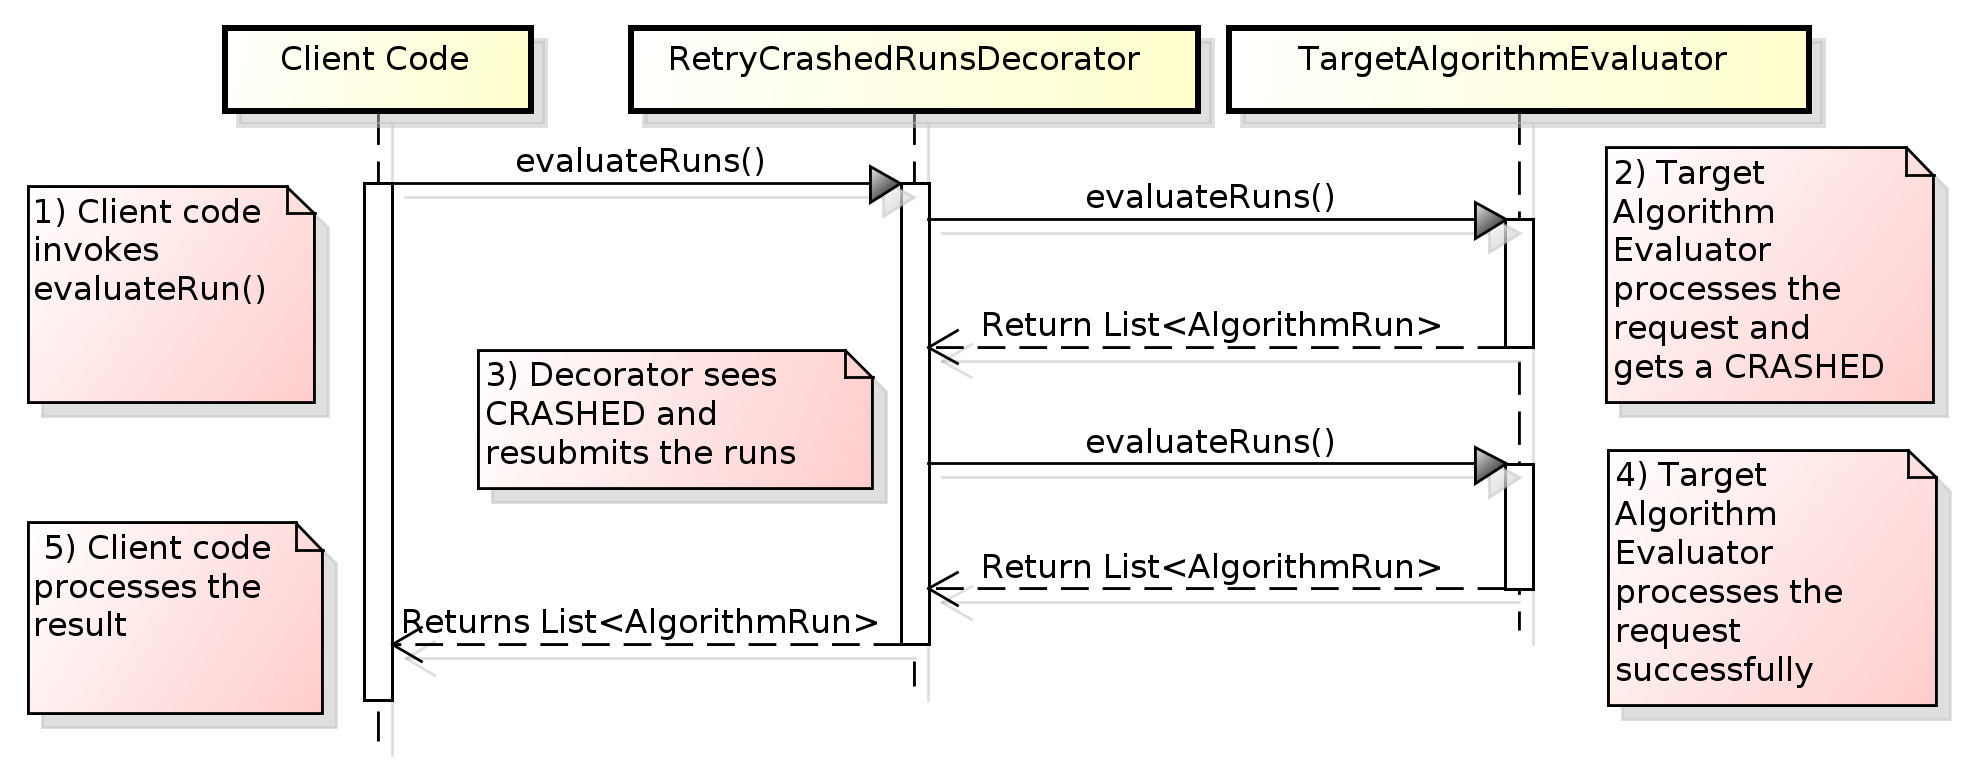
\includegraphics[scale=0.75]{img/UML/TAEDecoration.png}
\end{center}


\subsection{Decorator Types}

EALib includes over 20 decorators currently, and by default the \texttt{TargetAlgorithmEvaluator} returned by \texttt{getTargetAlgorithmEvaluator()} is decorated more than 6 times.

Different Decorators serve different purposes and can loosely be broken into different types. Please look at the javadoc for a full listing of all them:

\begin{description}
\item[Debugging Decorators] can help debugging by logging every run to screen or double check invariants. See the \texttt{ca.ubc.cs.beta.aclib.targetalgorithmevaluator.decorators.debug} package.
\item[Safety Decorators] check that the target algorithm or the client program is behaving correctly, for instance checking that the target algorithm always gives the same satisfiability response for an instance. See the\\ \texttt{ca.ubc.cs.beta.aclib.targetalgorithmevaluator.decorators.safety} package.
\item[Helpful Decorators] can transform the results of runs or do other processing, such as retrying crashed runs, generate reports of \texttt{TargetAlgorithmEvaluator} utilization. See the \\ \texttt{ca.ubc.cs.beta.aclib.targetalgorithmevaluator.decorators.helpers} package.
\item[Functionality Decorators] provide functionality for \texttt{TargetAlgorithmEvaluator} implementations so that they don't have to. For instance the \texttt{getNumberOfOutstandingEvaluations()} method is actually not implemented by any \texttt{TargetAlgorithmEvaluator} implementations, but by a single decorator. See the \\ \texttt{ca.ubc.cs.beta.aclib.targetalgorithmevaluator.decorators.functionality} package.
\item[Resource Management Decorators] allow you to limit different parts of your application to only emitting a certain number of runs at any given time. See the \\
\texttt{ca.ubc.cs.beta.aclib.targetalgorithmevaluator.decorators.resource} package.
\end{description}

Many of the decorators above can be applied automatically on the command line, others are applied internally when constructed, and others by the application itself depending on it's needs.

\subsubsection{Decorator Interactions}

The order in which decorators are applied does matter. Consider for the semantics of \\ \texttt{waitForOutstandingEvaluations()} which is a method that blocks until all outstanding runs are completed, for our purposes we will refer to the decorator that provides this as the OutstandingTAE. When coupled with the decorator that we saw in Section \ref{sec:decoration-example} (call it the RetryCrashedRunsTAE), it has different behaviour depending on the order.

\begin{enumerate}
\item If the OutstandingTAE is applied first, and the RetryCrashedRunsTAE wraps this, then a thread that calls \texttt{waitForOutstandingEvaluations()}, will return during the time that the RetryCrashedRunsTAE is deciding to continue.
\item If the RetryCrashRunsTAE is applied first, and then the OutstandingTAE applied second, then the method behaves as expected
\end{enumerate}

Another effect is that some decorators can nullify or invalidate the behaviour of other decorators. For instance if a decorator is enqueueing some runs, then the \texttt{waitForOutstandingEvaluations()} method if provided internally is simply broken. 

In general as a client you don't need to worry about this too much, the decorators returned by \texttt{getTargetAlgorithmEvaluator()} are provided in the correct order, and it's generally rare to write a new decorator with any complex functionality.

\subsection{Target Algorithm Evaluator Implementations}

\subsubsection{Built-in}

EALib includes several built-in Target Algorithm Evaluators. They are:

\begin{description}
\item[CLI] which invokes the wrapper directly.
\item[ANALYTIC] which uses a built in function to evaluate the \texttt{RunConfiguration}
\item[RANDOM] which generates random responses
\item[CONSTANT] which provides the same answer every time.
\item[PRELOAD] which allows you to supply a list of responses and they will be returned in order.
\end{description}

\subsubsection{Plugins}

EALib also supports plugins, that is other TAEs can be created and dropped into existing EALib based applications. This is done via dropping the required files in a subdirectory of the \texttt{plugins/} directory. The \texttt{plugins/} folder must be located next to the \texttt{ealib.jar} file on the classpath.

One existing plugin (and perhaps the only reason they exist) is the \texttt{MYSQLDB} plugin which allows any EALib application to distribute the jobs to a cluster via a MySQL database. The usage and evaluation of it is outside the scope of this document.

\subsubsection{Implementing Your Own TargetAlgorithmEvaluator}

Implementing your own Target Algorithm Evaluator and using it as a plugin in any EALib application is fairly simple but involves a few steps.

\textsc{Note}: This section is primarily about implementing new \texttt{TargetAlgorithmEvaluator}, if you would simply like a decorator to do something in your application, you can simply write it directly. Consider subtyping \texttt{AbstractTargetAlgorithmEvaluatorDecorator}.


\begin{center}
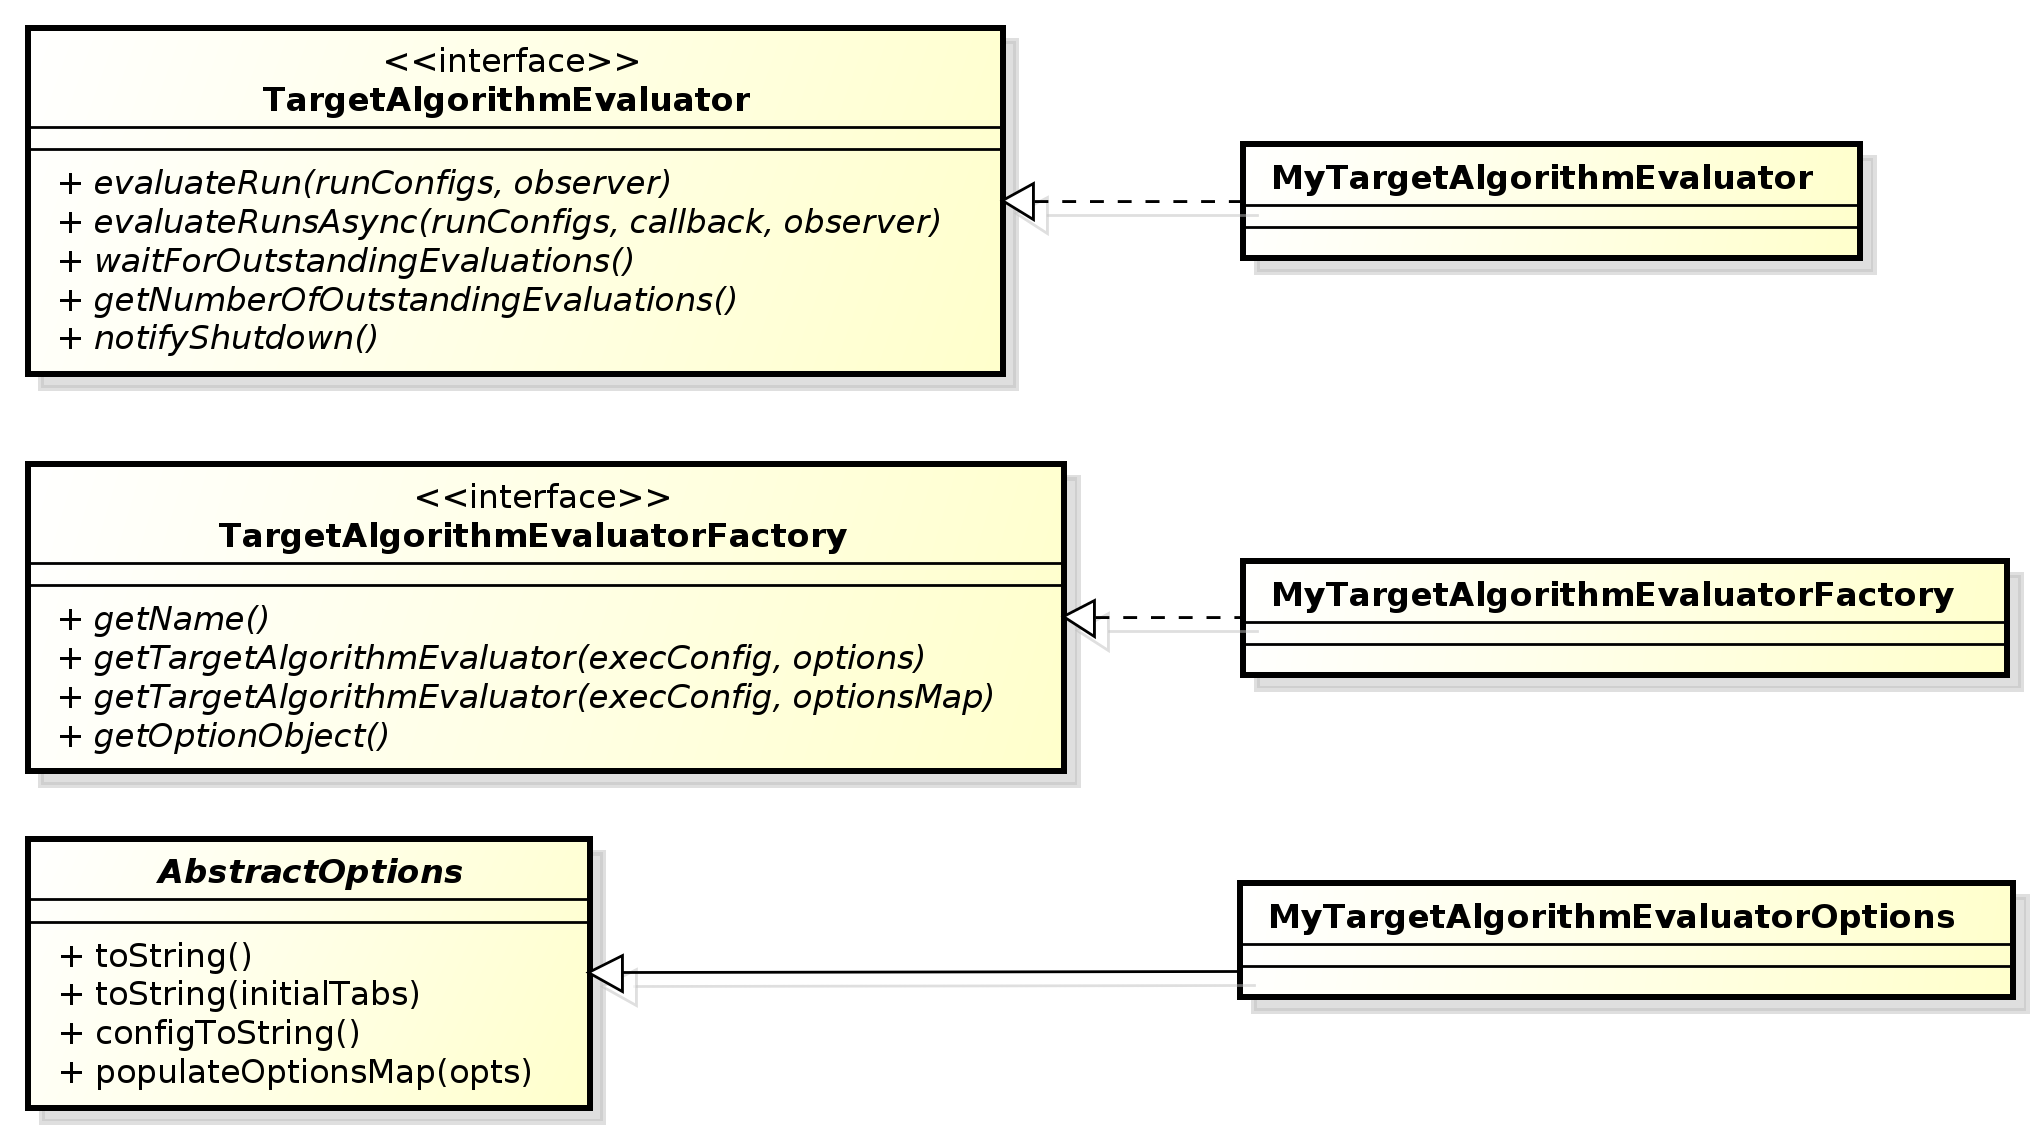
\includegraphics[scale=0.50]{img/UML/TAEFactory.png}
\end{center}

The first is that you need to actually provide the necessary classes of which there are three:

\begin{itemize}
\item You must have something that implements the \texttt{TargetAlgorithmEvaluator} interface.
\item You must have something that implements the \texttt{TargetAlgorithmEvaluatorFactory} interface, further it must have a no-argument constructor. The \texttt{getName()} method should return a string with no whitespace, that is in all capitals and is unique (for instance \textbf{CLI}). This name will be used to select your TAE on the command line. Additionally the constructor, the \texttt{getName()} and \texttt{getOptionsObject()}, cannot use or create a logger \footnote{If you try EALib will not load your TAE. The reason for this is that logging is configurable and at the point where we are asking for the name and options, we haven't configured anything}

\item If you would like to have any options on your implementation you will need to subtype \texttt{AbstractOptions}.
\end{itemize}


\begin{center}
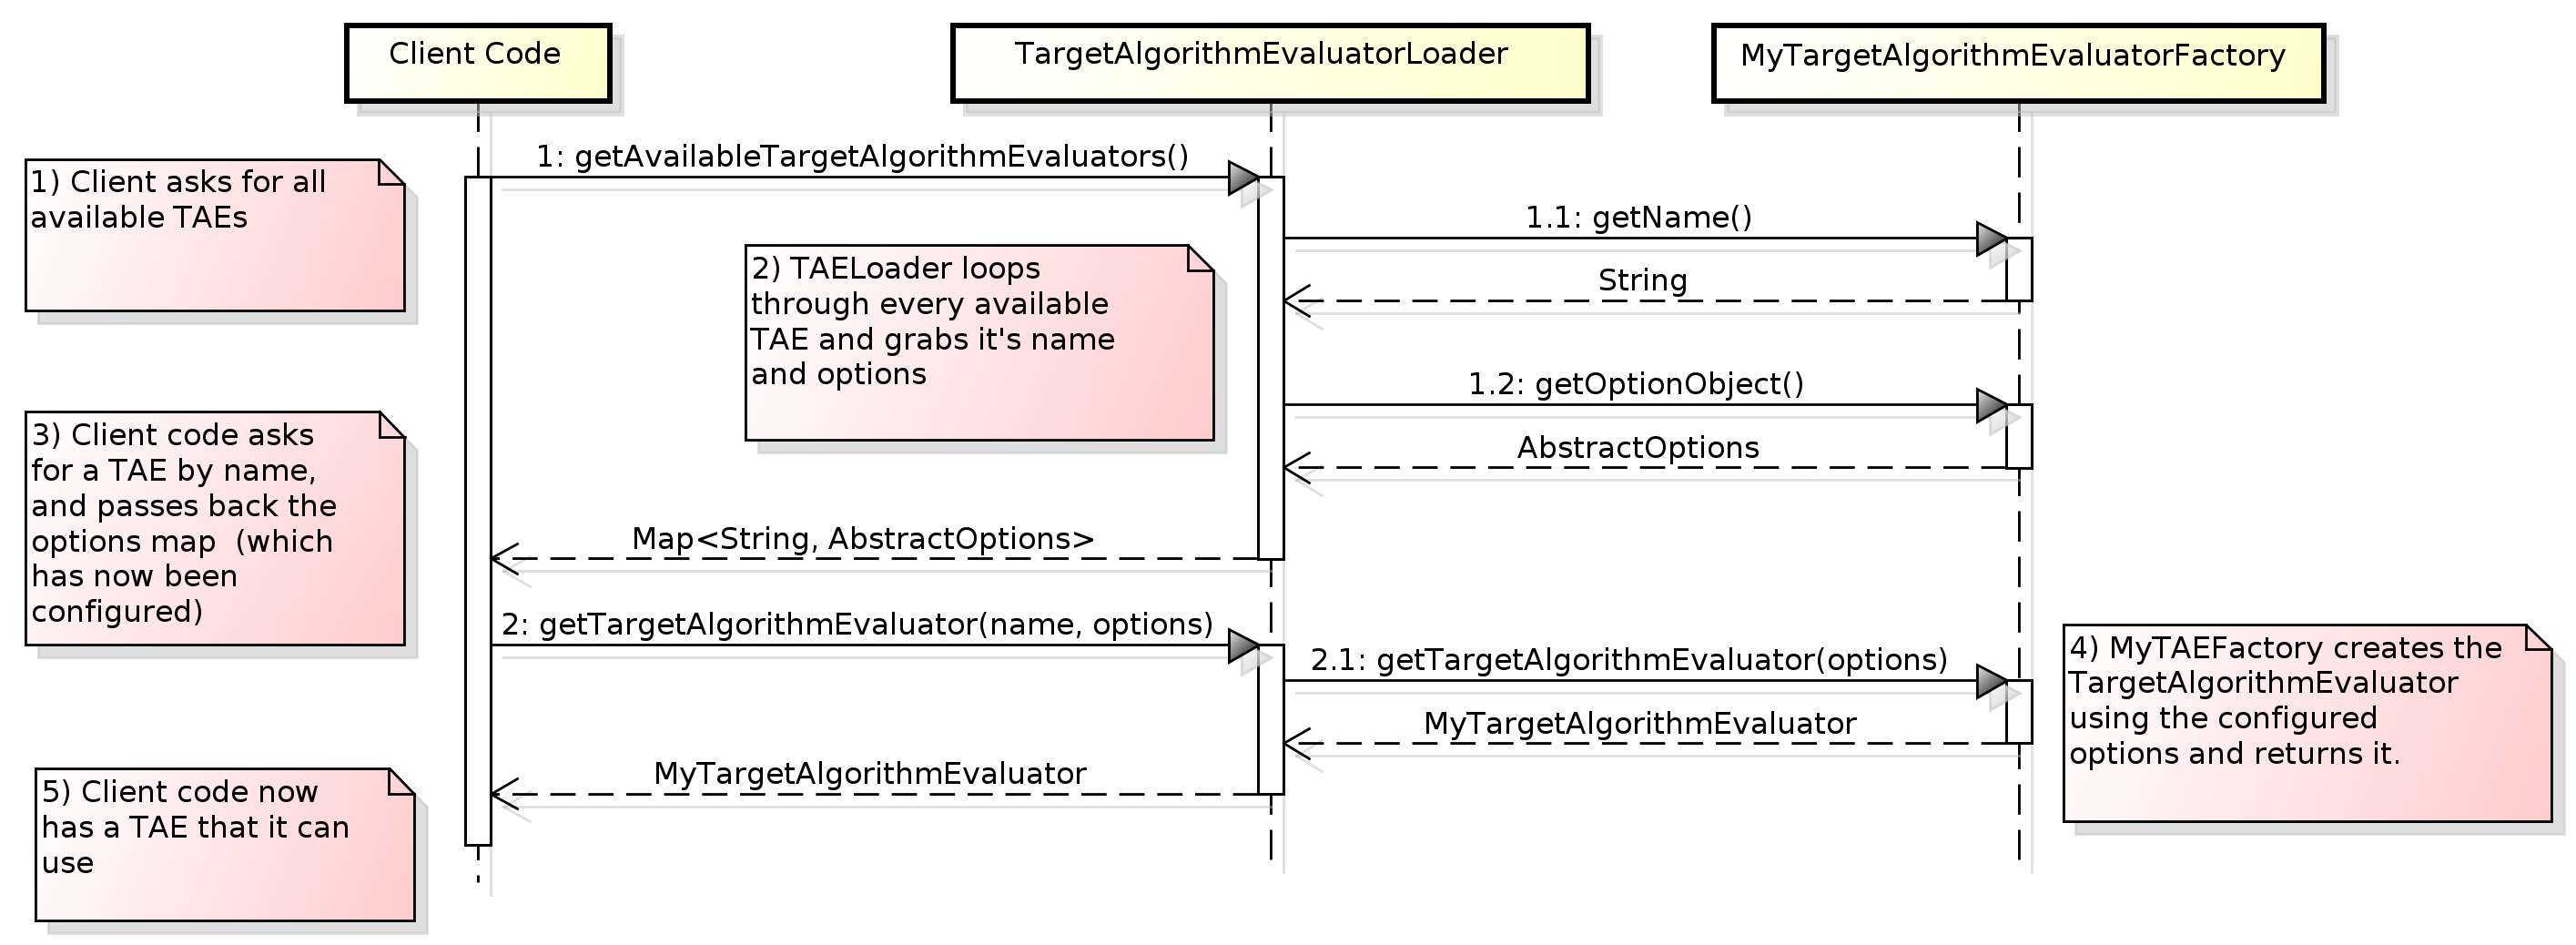
\includegraphics[scale=0.50]{img/UML/TAEConstruction.png}
\end{center}

\textsc{Note:} The above sequence diagram omits how the Decorators are applied, and doesn't show how the options are configured on the command line (which would happen after step 1 completes, but before step 2 begins).





Once you have your implementation you need to supply a jar that is configured with SPI (see Section \ref{sec:misc-spi}. 

If you are using eclipse the easiest way to do this is to use the spi-0.2.4.jar as follows:

\begin{enumerate} 
\item At the top of your \texttt{TargetAlgorithmEvaluatorFactory} class put the following annotation: \texttt{@ProviderFor(TargetAlgorithmEvaluatorFactory.class)}. (You will need to import the  \texttt{spi-0.2.4.jar} into your project to get the annotation.

\item Right click on your project in eclipse, and go to Properties $\rightarrow$Java Compiler$\rightarrow$Annotation Processing. Then click the button that says \emph{Enable annotation processing}.

\item Right click on your project in eclipse and go to Properties $\rightarrow$ Java Compiler $\rightarrow$Annotation Processing $\rightarrow$Factory Path, and hit \emph{Add JAR} button add the spi-0.2.4.jar.

\item If you are using Eclipse to build your JAR then when you are exporting you should check \emph{Export all ouptut folders for checked projects} on the first screen. 


\end{enumerate}

\textsc{TIP:} Regardless of whether you do it manually or automatically you can check if the JAR was built correctly by opening it (JAR files are simply zip files and checking that there is a folder \texttt{META-INF/services} in this folder should be a file named the canonical class name of \texttt{TargetAlgorithmEvaluatorFactory}. Opening that file should list the canonical name of your class on a line by itself.

\begin{center}
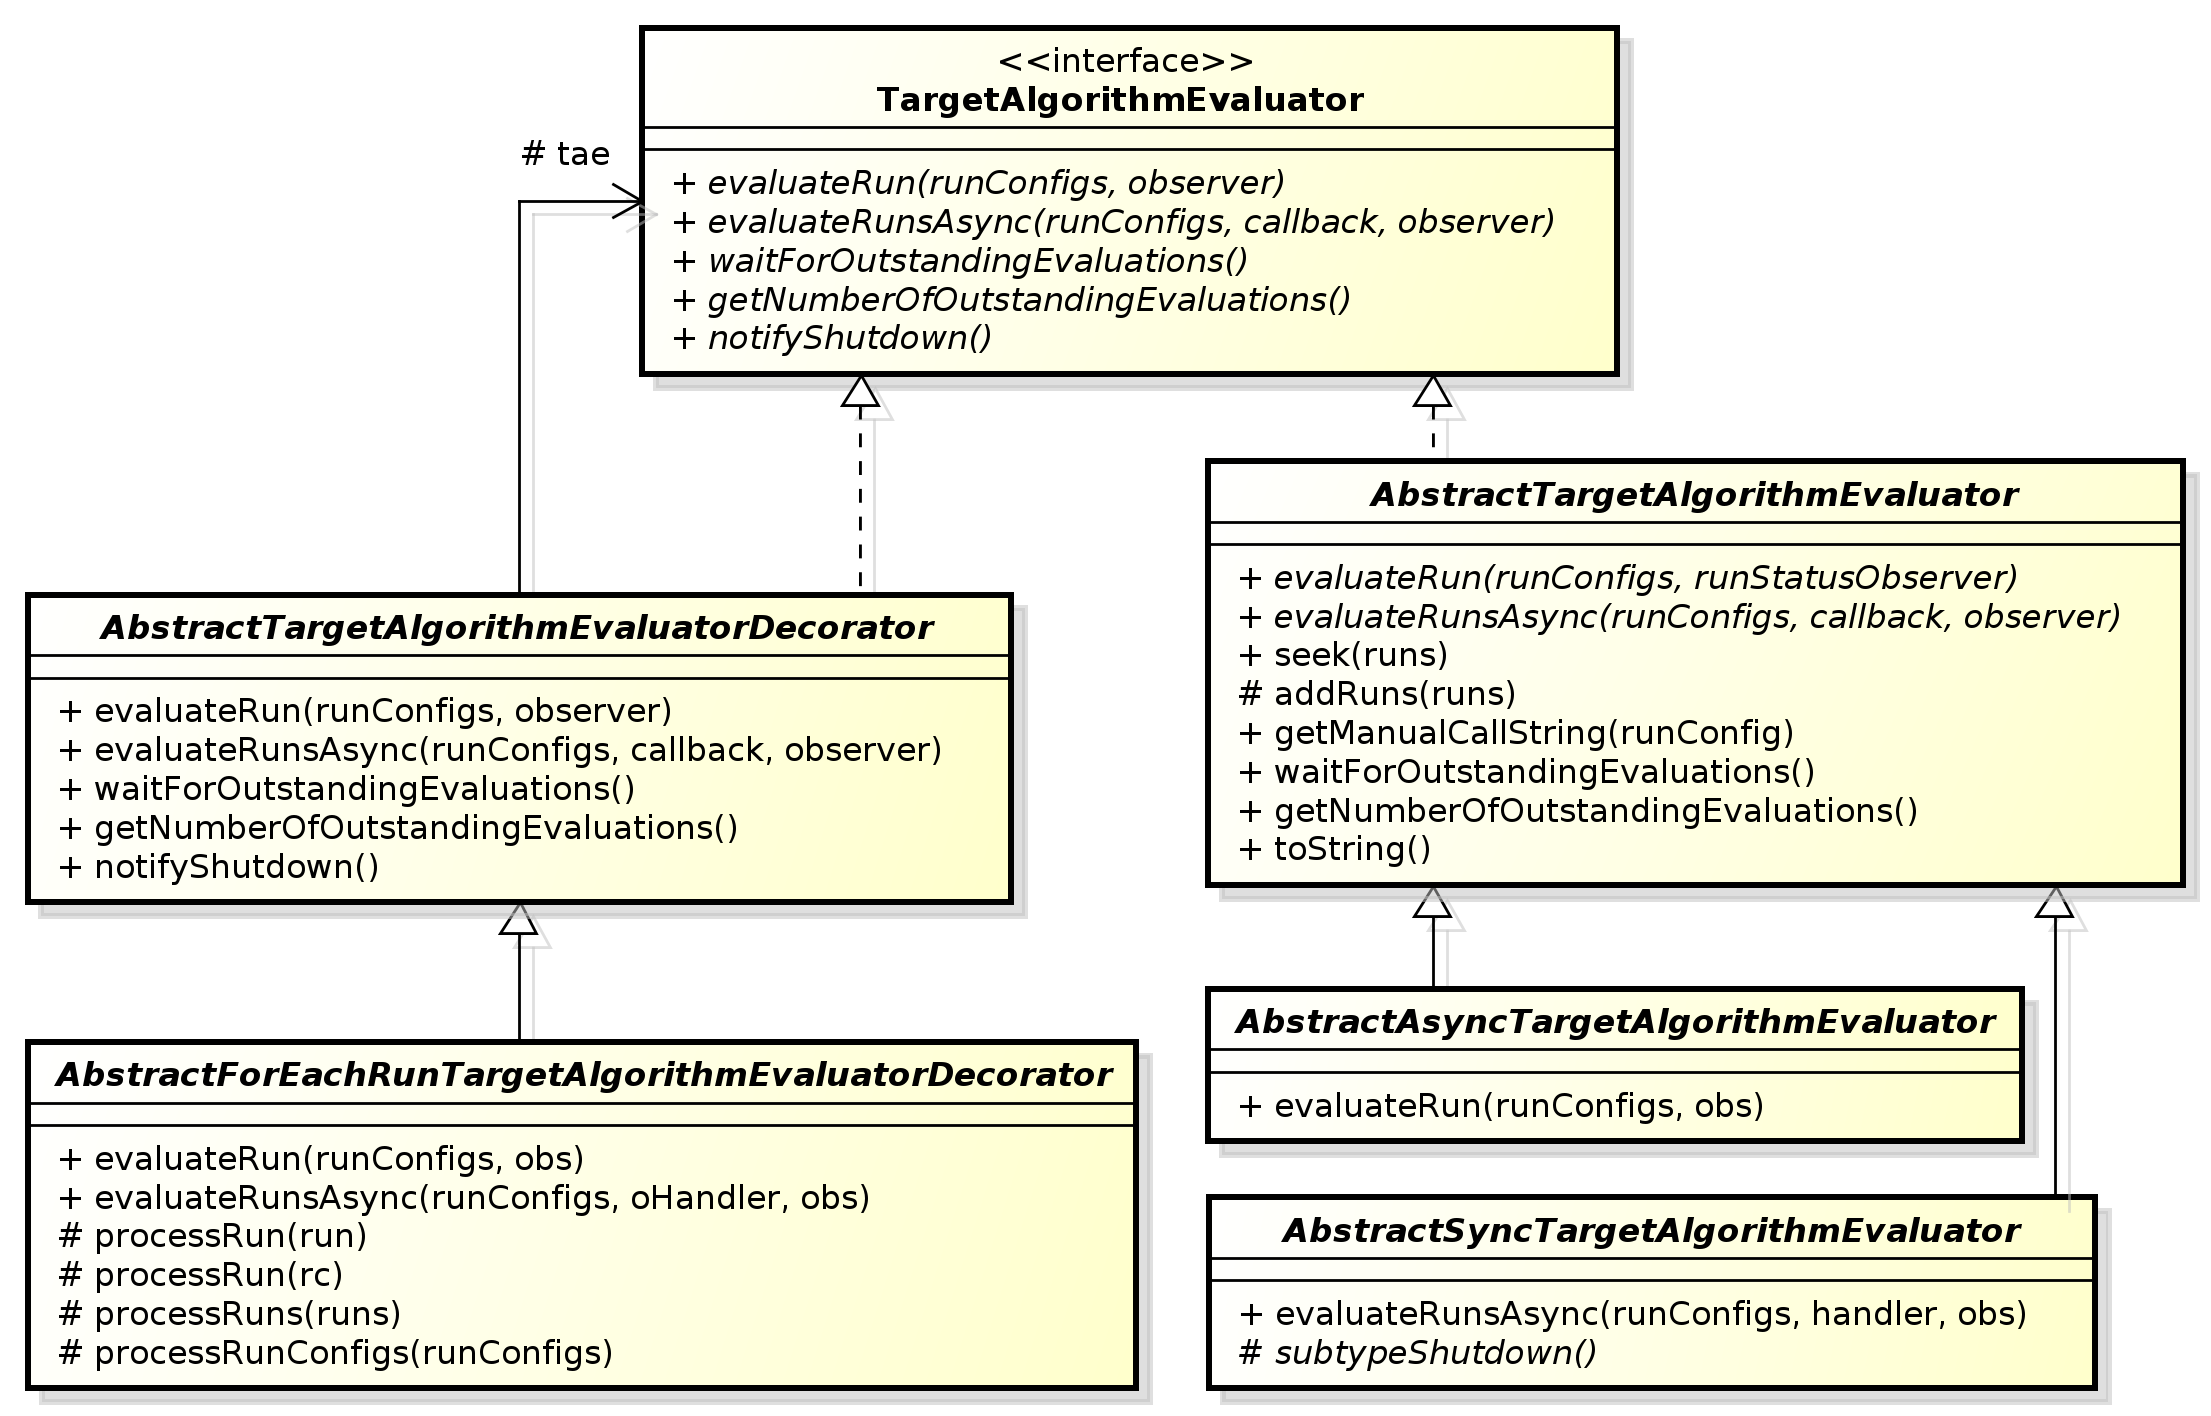
\includegraphics[scale=0.65]{img/UML/TAESubtypes.png}
\end{center}

There are a variety of different base types you can use if you would like to implement your own \texttt{TargetAlgorithmEvaluator}. Currently you can't easily add your own \texttt{TargetAlgorithmEvaluatorDecorator} but you can simulate it easily enough by having your own subtype be a decorator, and having an argument in your options be the actual \texttt{TargetAlgorithmEvaluator} users should use. \textsc{Note:} If you do this approach you should use the \texttt{TargetAlgorithmEvaluatorLoader} to get the base type as other methods (such as thhrough \texttt{TargetAlgorithmEvaluatorBuilder} and \texttt{TargetAlgorithmEvaluatorOptions} will cause decoration to occur twice which isn't what you want.

The different base types you can use differ in the following ways

\begin{description}

\item[TargetAlgorithmEvaluator] the raw interface and leaves you implementing everything yourself.

\item[AbstractTargetAlgorithmEvaluator] handles almost everything and leaves you to write the \texttt{evaluateRun()} and \texttt{evaluateRunAsync()} method.

\item[AbstractAsyncTargetAlgorithmEvaluator] requires you only to write the \texttt{evaluateRunAsync()} as the \texttt{evaluateRunSync()} method is automatically converted. This mechanism for handling both cases generally scales fine.

\item[AbstractSyncTargetAlgorithmEvaluator] requires you only to write the \texttt{evaluateRunSync()} method as the \texttt{evaluateRunAsync()} method simply launches a thread that invokes it synchronously. This mechanism for handling both cases generally scales poorly as it requires a new thread for every request.

\item[AbstractTargetAlgorithmEvaluatorDecorator] requires another \texttt{TargetAlgorithmEvaluator} in it's constructor. It simply delegates each method to the protected field \texttt{tae}. The \texttt{toString()} method is modified to return something useful.

\item[AbstractForEachRunTargetAlgorithmEvaluatorDecorator] like the previous example it requires another \texttt{TargetAlgorithmEvaluator} in it's constructor. However it has it's own internal \texttt{evaluateRun()} and \texttt{evaluateRunsAsync()} method, these methods invoke the protected methods \texttt{processRunConfigs()} and \texttt{processRunConfig()} prior to calling the wrapped decorator, allowing the runs to be processed / transformed before executing,
and then calls \texttt{processRuns()} and \texttt{processRun()} after the results are returned prior to returning them. This decorator can make it very easy to transform results.
\end{description}


\section{Miscellaneous}


\subsection{SPI}
\label{sec:misc-spi}

\subsection{Version}
\label{sec:version}



\section{Alex's Frequently Asked Questions}

\subsection{How can I use more than one instance of a particular ParametersDelegate in an application (say I want to parse multiple scenario files, or multiple instance lists)?}

\subsection{If I have many runs to do, how should I group batches?}

\subsection{I would like to use an EALib program as a plugin in another, is there a way for me to inject the TAE into it}.




%%%%%%%%%%%%%%%%%%%%%%%%%%%%%%%%%%%%%%%%%%%%%%%%%%%%%%%%%%%%%%%%%%%%
\section{Acknowledgements}
%%%%%%%%%%%%%%%%%%%%%%%%%%%%%%%%%%%%%%%%%%%%%%%%%%%%%%%%%%%%%%%%%%%%

We are indebted to Jonathan Shen for porting our random forest code from C to Java in preparation for a Java port of all of SMAC. We thank Marius Schneider for many valuable bug reports and suggestions for improvements. Thanks also to Chris Thornton, and Alexandre Fr\'echette for being a secondary beta testers.


\renewcommand{\bibsection}{\section{References}}
\bibliographystyle{apalike}
\bibliography{short,frankbib}


\end{document}

